\documentclass[11pt,oneside,a4paper]{article}
\usepackage[utf8]{inputenc}
\date{}
\usepackage[linesnumbered,ruled,vlined]{algorithm2e}
\SetKwInput{KwInput}{Input}                % Set the Input
\SetKwInput{KwOutput}{Output}              % set the Output<z
\usepackage{blindtext}
\usepackage{changepage}

\usepackage{amsmath}
\usepackage{color}

\usepackage{sectsty}
\usepackage{stmaryrd}
\usepackage{gensymb}
\usepackage{wasysym}
\usepackage{amsfonts}
\usepackage{xcolor}
\usepackage{graphicx}
\usepackage{stmaryrd}
\usepackage{mathtools}
\usepackage{amsthm}
\usepackage{caption}
\usepackage{subcaption}
%__________WIDE HAT_________
\usepackage{scalerel,stackengine}
\stackMath
\newcommand\reallywidehat[1]{%
\savestack{\tmpbox}{\stretchto{%
  \scaleto{%
    \scalerel*[\widthof{\ensuremath{#1}}]{\kern-.6pt\bigwedge\kern-.6pt}%
    {\rule[-\textheight/2]{1ex}{\textheight}}%WIDTH-LIMITED BIG WEDGE
  }{\textheight}%
}{0.5ex}}%
\stackon[1pt]{#1}{\tmpbox}%
}
\parskip 1ex
%______________________________

\setlength{\parindent}{0in}
\theoremstyle{definition}
\newtheorem{definition}{Definition}[section]

\theoremstyle{remark}
\newtheorem*{remark}{Remark}
\usepackage{amsmath}
\usepackage[T1]{fontenc}
\usepackage[colorlinks=true]{hyperref}
\usepackage{float}
\usepackage[british,UKenglish,swedish,USenglish,english,american]{babel}
\usepackage[T1]{fontenc}
\usepackage{fancyhdr}
\usepackage{natbib}
%\pagestyle{fancy}
\begin{document}
\renewcommand{\bibname}{References}
\hypersetup{citecolor=black}
\begin{titlepage}\centering
\vspace*{\fill}
\Huge Assignment 1\\
\vspace*{10mm}
\large Methods of PCA, MDS and Isomap \\
\vspace*{\fill}
\large \textsc{DD2434 Advanced Machine Learning} \\
\textsc{Filip Bergentoft, bergento@kth.se} \\
\end{titlepage}

\newpage

\section*{Problem 1}
Let $\theta = (\theta^r, \theta^e, \theta^a, \psi)$ and $X_{nlm} = 1$ if reader $n$ has clicked on advertisement $m$ in edition $l$, $X_{nlm} = 0$, otherwise.


The ECLL is given by

\begin{align*}
  ECLL = \sum_{nlm} \mathbb{E}_p(Z|)
\end{align*}










Given that we can observe both $Z$ and $X$ we get the following likelihood

\begin{align*}
  L(\theta; D) & = \prod_{n,l,m}p(X_{nlm}, Z_n^r, Z_l^r, Z_m^a | \psi) \\
  & = \prod_{nlm} \prod_{cdf} (\theta_c^r)^{ I(Z_n^r = c)} (\theta_d^e)^{ I(Z_l^e = d)}
  (\theta_f^a)^{ I(Z_m^a = f)} p(X_{nlm} |\psi_{cdf})^{I((Z_n^r, Z_l^r, Z_m^a) = (c,d,f)}
\end{align*}

Can now look at the log-likelihood

\begin{align*}
    l(\theta; D) & = \sum_{nlm}\sum_{cdf} I(Z_n^r = c) ln(\theta_c^r) + I(Z_l^e = d) ln(\theta_d^e)
    + I(Z_m^a = f) ln(\theta_f^a) \\
    & + I((Z_n^r, Z_l^r, Z_m^a) = (c,d,f)) ln(p(X_{nlm} |\psi_{cdf}))
\end{align*}

Now let

\begin{align*}
  & A = \sum_{cdf}\sum_{nlm} I(Z_n^r = c) ln(\theta_c^r) + I(Z_l^e = d) ln(\theta_d^e)
  + I(Z_m^a = f) ln(\theta_f^a) \\
  & B = \sum_{nlm}\sum_{cdf} I((Z_n^r, Z_l^r, Z_m^a) = (c,d,f)) ln(p(X_{nlm} |\psi_{cdf}))
\end{align*}

Can then rewrite $A$ in the following manner

\begin{align*}
  A = \sum_{cdf} LM N_c^r ln(\theta_c^r) + NM N_d^e ln(\theta_d^e) + NL ln(\theta_f^a)
\end{align*}

Where each term can be maximised independently using known techniques from lectures yielding

\begin{align*}
  & \theta_c^r = \frac{N^r_c}{N} \\
  & \theta_d^e = \frac{N^e_d}{L} \\
  & \theta_c^r = \frac{N^a_f}{M}
\end{align*}


\section*{2.2 Likelihood of a Tree Graphical Model}


\begin{tcolorbox}
\textbf{Question 2.2.7:}
Implement a dynamic programming algorithm that, for a given $T, \Theta \text{ and } \beta$ computes $p(\beta | T, \Theta)$
\end{tcolorbox}

$T$ is a binary tree with a vertex set $V(T)$ and a leaf set $L(T)$. For each vertex $v \in V(T)$ there is an associated random variable $X_v \in [K]$ with a corresponding CPD $\theta_v = p(X_v|x_{pa(v)})$ which is a categorical distribution. $\beta$ is defined as the set of values of all leafs in $T$ such that $\beta = \{x_l \, : \, l \in L(T)$.

In order to compute $p(\beta | T, \Theta)$ we need to find an expression that can be used for dynamic programming, I.E. splitting up the full problem into smaller subproblems. By looking at the definition of $s$ in equation (\ref{def_s})

\begin{equation}
  s(u,i) = p(X_{Observed \, \cap \, \downarrow u}| X_u = i)
  \label{def_s}
\end{equation}

and letting the root node of the tree being denoted by $r$, one can use that if $u$ is chosen as the root $r$ we get the following expression

\begin{align*}
  s(r,i) = p(X_{Observed \, \cap \, \downarrow r}| X_r = i) = \bigg\{ X_{Observed \, \cap \, \downarrow r} = \beta \bigg\} = p(\beta | X_r = i, T, \Theta)
\end{align*}

We can then marginalise this using Bayes' theorem in the following manner

\begin{align}
  p(\beta | T, \Theta) & = \sum_i p(\beta, X_r = i| T, \Theta) = \sum_i p(\beta | X_r = i, T, \Theta)p(X_r = i) \\
  & = \sum_i s(r,i)p(X_r = i)
  \label{sol_eq}
\end{align}

Using that $T$ is a binary tree and thus if $v, w$ are children to a node $u$ then

\begin{align}
  s(u,i) & = p(X_{Observed \, \cap \, \downarrow u}| X_u = i)\nonumber \\
  & = p(X_{Observed \, \cap \, \downarrow v}| X_v = i)
  p(X_{Observed \, \cap \, \downarrow w}| X_w = i) \nonumber\\
  & = \bigg( \sum_j s(v,j)p(X_v = j| x_u = i) \bigg )\bigg( \sum_j s(w,j)p(X_w = j| x_w = i) \bigg )
  \label{traverse_eq}
\end{align}

A special case is when the node $u$ is a leaf node, then the following holds

\begin{align}
  s(u,i) = \begin{cases} 1, & X_u = i \\ 0, & otherwise\end{cases}
  \label{eq_3}
\end{align}


Equation (\ref{sol_eq}) can then be computed using dynamic programming by starting at the leaf nodes using equation (\ref{eq_3}) and then traversing up the nodes in the tree to the root using equation (\ref{traverse_eq}) one level at a time and storing the achieved probabilities $s$ along the way.
\\

\begin{tcolorbox}
\textbf{Question 2.2.8:}
Apply your algorithm to the graphical model and data provided separately
\end{tcolorbox}

The following likelihoods were achieved when applying my implementation of the dynamic programming algorithm on the given trees.


\begin{center}
    \begin{tabular}{ | c | c | c |  c | c | c |}
    \hline
    Tree sample: & $0$ & $1$ & $2$ & $3$ & $4$ \\ \hline
    Small tree & $0.016$ & $0.015$ & $0.011$ & $0.007$ & $0.041$ \\ \hline
    Medium tree & $4.336 \cdot 10^{-18}$ & $3.094 \cdot 10^{-20}$ & $1.050 \cdot 10^{-16}$ & $6.585 \cdot 10^{-16}$ & $1.488 \cdot 10^{-18}$ \\ \hline
    Large tree & $3.288 \cdot 10^{-69}$ & $1.109 \cdot 10^{-66}$ & $2.522 \cdot 10^{-68}$ & $1.242 \cdot 10^{-66}$ & $3.535 \cdot 10^{-69}$ \\ \hline
    \end{tabular}
\end{center}


\section*{Problem 3}
Want to maximise the expression $tr(Y^T W W^T Y)$ where $Y \in \mathbb{R}^{d \times n}$,
 $W \in \mathbb{R}^{d \times k}, \; k < d$ under the condition that $W$ has orthonormal columns which implies that $W^T W = I_k$. In order to achieve this we want to use Lagrange multipliers, and for mathematical convenience we will use the cyclic property of trace to shift around the matrices in the expression in the following manner.

 \begin{equation}
   tr(Y^T W W^T Y) =  tr(Y Y^T W W^T) = tr(W^T Y Y^T W)
 \end{equation}

We thus want to maximise $tr(W^T Y Y^T W)$ subject to $W^T W - I_k = 0$ which yields the following Lagrangian function

\begin{align}
  L & = tr(W^T Y Y^T W) - \sum_{i = 1}^k \sum_{j = 1}^k \lambda_{ij}(w_i^T w_j - \mathbf{1} \{i = j \}) \\
  & = \sum_{i = 1}^k w_i^T Y Y^T w_i - \sum_{i = 1}^k \sum_{j = 1}^k \lambda_{ij}(w_i^T w_j - \mathbf{1} \{i = j \})
\end{align}

where $\mathbf{1}$ is the indicator function.

Taking the derivative with respect to the $\lambda_{lj}$ only results in the initially stated condition that

\begin{align}
  W^T W = I_k
  \label{cond_1}
\end{align}

Taking the derivative with respect to $w_l, \; l = 1,..., k$ yields

\begin{align}
  \frac{\partial L}{\partial w_l} & = 2 Y Y^T w_l - \sum_{j = 1}^k (\lambda_{lj} w_j + \lambda_{jl} w_j) = 0
  \label{3_1}
\end{align}

By letting $\Lambda$ be a matrix with elements $(\Lambda)_{lj} = \lambda_{lj}$ equation (\ref{3_1}) can be expressed using matrices for all $l = 1,..., n$.

\begin{align}
  2 Y Y^T W - W(\Lambda^T + \Lambda) = 0 \Rightarrow Y Y^T W = W \; \frac{\Lambda^T + \Lambda}{2}
  \label{3_2}
\end{align}

Noting that $\frac{\Lambda^T + \Lambda}{2}$ is trivially symmetric it can be diagonalised in the following manner: $\frac{\Lambda^T + \Lambda}{2} = PDP^{-1}$. Substituting this into equation (\ref{3_2}) results in

\begin{align}
  & Y Y^T W = W \; \frac{\Lambda^T + \Lambda}{2} = W PDP^{-1} \\
  & \Rightarrow  W^T Y Y^T W = W^T W PDP^{-1} = \bigg\{ W^T W = I_k \text{ by } (\ref{cond_1})\bigg\} = PDP^{-1} \\
  \label{3_3}
  & \Rightarrow P^{-1} W^T Y Y^T W P = P^{-1} PDP^{-1} P \\
  & \Rightarrow P^{-1}W^T Y Y^T WP = D
\end{align}

Thus is $Y Y^T$ diagonalised by $WP$ and $D$ thus consist of $k$ eigenvalues of $Y Y^T$ and by substituting equation (\ref{3_3}) into the original trace expression we get

\begin{align}
  tr(W^T Y Y^T W) = tr(PDP^{-1}) = tr(P^{-1} P D) = tr(D) = \sum_{i=1}^k d_i
\end{align}

where $d_i$ are eigenvalues of $Y Y^T$. Thus in order to maximise this we just choose $d_i, i = 1,2,...,k$ to be the $k$ largest eigenvalues of $Y Y^T$.

Now to show that if we select $W = U_k$ we get the same maximum value. Using the skinny SVD of $Y = U \Sigma V^T$ and substituting into the original trace expression we get

\begin{align}
  tr(Y^T W W^T Y) & = tr(V \Sigma^T U^T W W^T U \Sigma V^T) \\
  & = tr(V^TV \Sigma U^T W W^T U \Sigma) = tr(\Sigma U^T W W^T U \Sigma) \\
  & = tr(\Sigma U^T U_k U_k^T U \Sigma) = tr((\Sigma U^T U_k) (\Sigma U^T U_k)^T) \\
  & = tr((\Sigma I_{d \times k}) (\Sigma I_{d \times k})^T) = tr{\Sigma_{kxk}^2} \\
  & = \sum_{i=1}^k \sigma_i^2 = \bigg\{k \text{ largest singular values} \bigg\} = \sum_{i=1}^k d_i
\end{align}


Thus is $tr(W^T Y Y^T W)$ subject to $W^T W - I_k = 0$ maximised by choosing $W = U_k$ and the maximum value is given by $\sum_{i=1}^k \sigma_i^2$.


\section*{2.4 Mixture of trees with observable variables}

\begin{tcolorbox}
\textbf{Question 2.4.12:}
Implement this EM algorithm.
\end{tcolorbox}
The EM algorithm with sieving was was implemented in the following manner using the given Tree package.

\begin{algorithm}[H]
\SetAlgoLined
\KwInput{Data samples}
\KwOutput{Tree mixture}

  Compute a distance matrix of the data: $D \gets \text{weighted\_distance} (Y) $

  Compute a similarity matrix from $D$: $S \gets \text{similarity\_matrix} (D) $

  Compute Eigen-decomposition of $S$: $[D,Q] \gets \text{Eig}(S)$

  Order $D$ in descending order of eigenvalues magnitude and $Q$ correspondingly

  Ensure elements of $D$ and $Q$ are real

  Compute embedding: $X \gets I_{2\times 101}D Q^T$

  \caption{EM algorithm}
\end{algorithm}

\begin{tcolorbox}
\textbf{Question 2.4.13:}
Apply your algorithm to the provided data and show how well you reconstruct the mixtures. First, compare the real and inferred trees with the unweighted Robinson-Foulds (aka symmetric difference) metric. Do the trees have similar structure? Then, compare the likelihoods of real and inferred mixtures.
\end{tcolorbox}

\begin{tcolorbox}
\textbf{Question 2.4.14:}
Simulate new tree mixtures with different number of nodes, samples and clusters. Try to find some interesting cases. Analyse your results as in the previous question.
\end{tcolorbox}


\section*{Problem 5}


We are considering the classical MDS when $Y \in \mathbb{R}^{d \times n}$ is known which implies that we can construct a similarity matrix $S = Y^T Y$. An MDS embedding can then be obtained by performing eigen-decomposition on $S$ which yields the following

\begin{equation}
  S = Y^T Y = Q \Lambda Q^T = (\Lambda^{-\frac{1}{2}}Q^T)^T(\Lambda^{-\frac{1}{2}}Q^T)
\end{equation}

where $\Lambda$ is a diagonal matrix with eigenvalues of $S = Y^T Y$ sorted in descending order.

The latent matrix $X$ can then be chosen as

\begin{equation}
  X = I_{k \times n} \Lambda^{-\frac{1}{2}}Q^T , \; k < d
\end{equation}

However, this can also be written in terms of the SVD of $Y = U \Sigma V^T$

\begin{align}
  S & = Y^T Y = V \Sigma^T U^T U \Sigma V^T = V \Sigma^T \Sigma V^T = (\Sigma V^T)^T(\Sigma V^T) \\
  & = (\Lambda^{-\frac{1}{2}}Q^T)^T(\Lambda^{-\frac{1}{2}}Q^T)
\end{align}
Since $\Lambda$ and $\Sigma$ has ordered diagonals by magnitude and $V$ contains the right singular vectors we know that $V = Q$ which gives that
\begin{equation}
  \Lambda^{-\frac{1}{2}}Q^T = \Sigma V^T
\end{equation}

Thus can the latent matrix also be expressed as

\begin{equation}
  X = I_{k \times n} \Sigma V^T , \; k < d
  \label{5_1}
\end{equation}

In PCA we decompose $Y$ into its SVD, yielding

\begin{equation}
  Y = U \Sigma V^T
\end{equation}

The latent matrix is then chosen as

\begin{align}
  X & = (U I_{n \times k})^T Y = I_{k \times n} U^T Y \\
  & =  \bigg\{Y = U \Sigma V^T \Rightarrow U^T Y = \Sigma V^T \bigg\} \\
  & = I_{k \times n} \Sigma V^T , \; k < d
  \label{5_2}
\end{align}

Comparing equations (\ref{5_1}) and (\ref{5_2}) we see that the results are equivalent. \\

Regarding the computational efficiency I believe that there are two areas to consider: computational complexity and numerical accuracy. The complexities of computing the SVD and eigen-decomposition are similar and somewhat dependant on the properties of the input matrix, eigen-decomposition often performing a bit better. However, for the MDS we are required to perform a matrix multiplication beforehand which both introduces additional cost in time but can also introduce issues with numerical accuracy causing the resulting eigen-decomposition to have imaginary parts. For this reason the SVD should be preferred. 


\section*{3.6 Spectral Graph Analysis}
\begin{tcolorbox}
  \textbf{Problem formulation:} In this problem, you should solve each of the following three subproblems.

  \begin{itemize}
    \item Let $G=(V, E)$ be an undirected $d$-regular graph, let $A$ be the adjacency matrix of $G,$ and let $L=I-\frac{1}{d} A$ be the normalized Laplacian of $G .$ Prove that for any vector $\mathbf{x} \in \mathbb{R}^{|V|}$ it is
    \begin{equation}
      \mathbf{x}^{T} L \mathbf{x}=\frac{1}{d} \sum_{(u, v) \in E}\left(x_{u}-x_{v}\right)^{2}
      \label{spectral_expression}
    \end{equation}
    \item Show that the normalised Laplacian is a positive semidefinite matrix.
    \item Assume that we find a non-trivial vector $\mathbf{x}_{*}$ that minimises the expression $\mathbf{x}^{T} L \mathbf{x} .$ First explain what non-trivial means. Second explain how $\mathbf{x}_{*}$ can be used as an embedding of the vertices of the graph into the real line. Use Equation \eqref{spectral_expression} to justify the claim that $\mathbf{x}_{*}$ provides a meaningful embedding.
  \end{itemize}
\end{tcolorbox}

We begin by stating some useful properties that will be used throughout the problem. Given that $G=(V, E)$ is an undirected $d$-regular graph and that $A$ is an adjacency matrix it follows that

\begin{itemize}
  \item $A$ is symmetric
  \item $(A)_{uv} = a_{uv} = \begin{cases} 1, & (u,v) \in E \\ 0, & \text{otherwise}\end{cases}$
  \item Each row/column of $A$ sums up to $d$, I.E. $d = \sum_i{a_{ij}} = \sum_j{a_{ij}}$
  \item The main diagonal of $A$ is filled with zeros

\end{itemize}

\subsection*{First subproblem}

We can now begin the proof of the first subproblem.
\begin{align*}
  x^T L x & = x^T(I-\frac{A}{d})x = \frac{1}{d} x^T (dI - A) x = \frac{1}{d} (\sum_i d x_i^2 - \sum_{i,j}x_i a_{ij} x_j)
\end{align*}
Can now substitute for $d = \sum_j{a_{ij}}$ which yields that
\begin{align*}
  x^T L x & = \frac{1}{d} (\sum_{i,j} a_{ij} x_i^2 - \sum_{i,j}x_i a_{ij} x_j) \\
  & = \frac{1}{2d} (\sum_{i,j} a_{ij} x_i^2 + \sum_{i,j} a_{ij} x_j^2 - 2\sum_{i,j}x_i a_{ij} x_j) \\
  & = \frac{1}{2d} \sum_{i,j} a_{ij}(x_i-x_j)^2
\end{align*}
Using that $A$ is symmetric, I.E. that $a_{ij} = a_{ji}$ and that $a_{ii} = 0, \; \forall i$ we get that
\begin{align}
  x^T L x & = \frac{1}{2d} \sum_{i,j} a_{ij}(x_i-x_j)^2 \nonumber \\
  & = \frac{2}{2d} \sum_{i>j} a_{ij}(x_i-x_j)^2 \label{graph1} \\
  & = \frac{1}{d} \sum_{(i,j) \in E} (x_i-x_j)^2 \label{graph2}
\end{align}
where we between Equation \eqref{graph1} and Equation \eqref{graph2} used that $a_{uv} = \begin{cases} 1, & (u,v) \in E \\ 0, & \text{otherwise}\end{cases}$. Which was to proven.

\subsection*{Second subproblem}
We can now use the result of the first subproblem to show the second subproblem where we want to show that $L$ is a positive semi-definite matrix. I.E. that
\begin{equation}
  x^T L x \geq 0 \; \forall x \in \mathbb{R}^{|V|}
\end{equation}
In the first subproblem we showed that
\begin{equation}
  x^T L x = \frac{1}{d} \sum_{(i,j) \in E} a_{ij}(x_i-x_j)^2
  \label{second_sub}
\end{equation}
where $d$ is a positive integer and $x \in \mathbb{R}^{|V|}$. It is thus sufficient to show that equation \eqref{second_sub} is non-negative. Using that $f(t) = t^2$ is a non-negative function for all $t \in \mathbb{R}$. $x^T L x$ is thus a sum of non-negative values multiplied with a positive value $\frac{1}{d}$ which gives that
\begin{equation}
  x^T L x = \frac{1}{d} \sum_{(i,j) \in E} a_{ij}(x_i-x_j)^2 \geq 0
\end{equation}
Which in turn proves that $L$ is positive semi-definite.

\subsection*{Third subproblem}
In this problem a \textit{trivial} vector would be a constant vector I.E. that all elements in the vector are equal. This is since a constant vector will always minimise equation \eqref{spectral_expression}. Thus is, in this setting, a \textit{non-trivial} vector $x_*$ a non-constant vector. \\

In order to answer the second part of this question we need to understand what a \textit{meaningful embedding} corresponds to in this setting. One of the main uses of spectral graph analysis is to perform spectral clustering, where one aims to cluster points that are similar. A way of measuring similarity within a set of points is by the number of edges within that set, where more edges are better. A meaningful embedding would thus correspond to a way of clustering points such that the number of edges within the clusters are high.\\

We are given that $x_*$ is a non-trivial vector that minimises equation \eqref{spectral_expression}, $x_*$ is thus not a constant vector. So given that a non-constant $x_*$ vector is the solution to
\begin{equation}
  x_* = \underset{x}{\text{argmin }} \frac{1}{d} \sum_{(u, v) \in E}\left(x_{u}-x_{v}\right)^{2}
\end{equation}
where the sum is taken over the vertices $(u, v) \in E$, I.E. the vertices that have an edge between them. Given that a cluster of points is a set of points that have a lot of edges within that set, equation \eqref{spectral_expression} will be minimised if points in the same clusters have similar values for their corresponding element in $x_*$. Additionally, since we are seeking a non-trivial solution, points from different clusters will have different values for their corresponding element in $x_*$. Thus can one plot the elements of $x_*$ on the real line in order to receive a meaningful embedding. This will result in clusters of points on the real line representing clusters of the real data. \\

Note that if several vectors $x_1, x_2, ..., x_m$ minimises \eqref{spectral_expression} (has small corresponding eigenvalues), one can apply k-means to those vectors to get a more accurate representation of the actual clusters that exist in the data.


\section*{Problem 7 - \href{https://github.com/Filipbergentoft/DD2434/tree/main/Assignment%201}{Link to GitHub}}


The goal of this problem is to visualise how similar different animals at a zoo are by projecting the given data from $\mathbb{R}^{16}$ to $\mathbb{R}^{2}$ using three different embeddings; PCA, MDS and Isomap. The data matrix $Y$ will be structured in the same way as in the lecture such that a column of $Y$ corresponds to a data point, thus is $Y \in R^{16 \times 101}$ as there are $101$ data points.

\subsection*{Preprocessing the data}
In order to enable the applications of the embeddings the data has to be preprocessed by first removing the columns 'type' and 'animal name' from the data set. These can later be used in the visualisation.

The remaining attributes are all boolean with values in $\{ 0,1 \}$ except the attribute 'legs' which takes values in $\{ 0, 2, 4, 6, 8 \}$. This attribute thus takes on values up to $8$ times the magnitude in comparison to the remaining attributes which results in the legs attribute to be seen as more important for the embeddings. For this reason the magnitude of 'legs' will be scaled down by $8$ times, causing it to instead take values in  $\{ 0, \frac{1}{4}, \frac{1}{2}, \frac{3}{4}, 1 \}$ giving it a similar magnitude to the remaining attributes.

\subsection*{Visualisation of data}
In order to project the data in 2D such that similar animals are projected close to one another the first two resulting latent variables from a method will be plotted against each other as they contain the most information about the data set as a result of the sorting of the singular values and eigenvalues in descending order.


\subsection*{PCA}
The implementation of PCA was solved in the following manner

\begin{algorithm}[H]
\SetAlgoLined
\KwInput{Data matrix $Y$}
\KwOutput{2-dimensional embedding $X$ }
\KwData{Zoo animals}
 Center the columns (data points) of the data matrix: $Y_c \gets \text{center}(Y)$

 Compute SVD of $Y_c$: $[U,\Sigma, V] \gets \text{SVD}(Y_c)$

 Select the first two columns of $U$: $W \gets [u_1, u_2]$

Compute embedding: $X \gets W^T Y_c$
 \caption{PCA method}
\end{algorithm}


The implementation was quite short using Numpy's Singular Value Decomposition function. The only concern that arised was the centring of the data matrix as it removes the boolean nature of the matrix. However I argue that this only translates the data points and does not remove the information of the attributes which renders the action viable.
\\

The following visualisation was achieved

\begin{figure}[H]
  \centering
  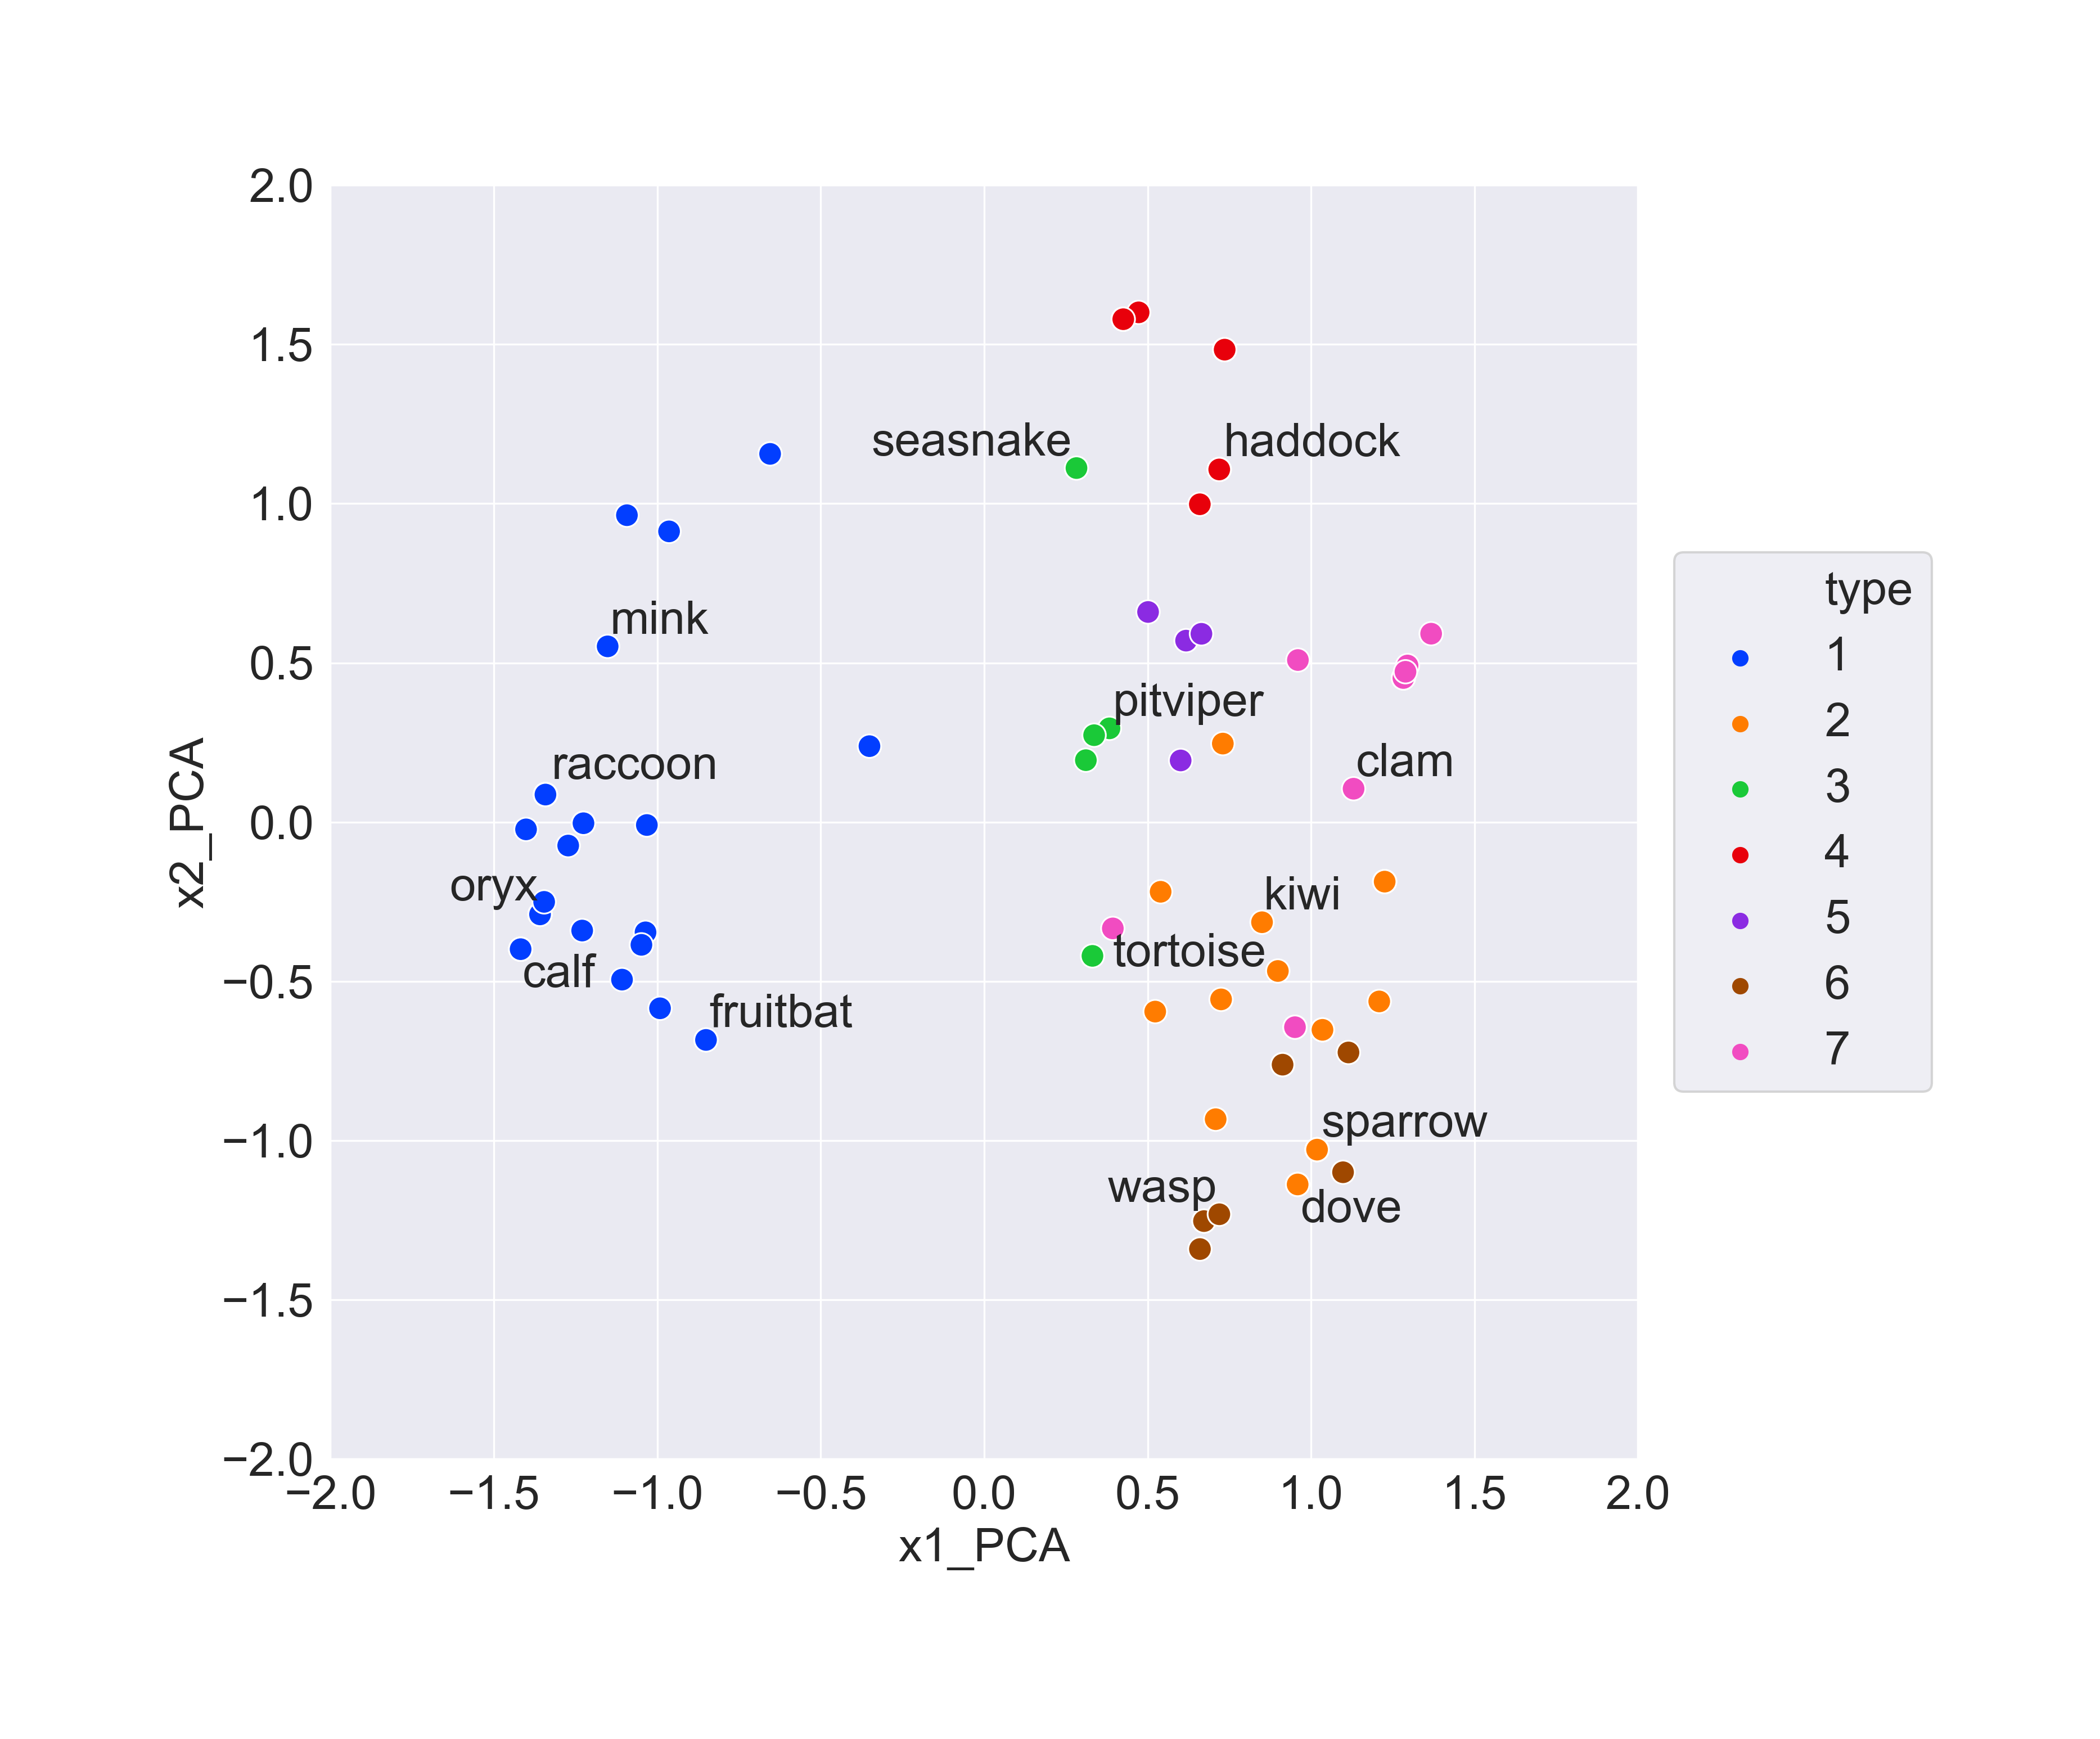
\includegraphics[width = 0.8\linewidth]{../Visualization_PCA.png}
  \caption{Visualisation PCA}
  \label{vis_PCA}
\end{figure}

where a few animals are annotated to give some intuition and understanding behind the placing of the different animals. It is apparent from the plot that there is a clear distinction between type $1$ and the remaining types $2-7$ whom are more mixed among each other.


\subsection*{MDS}
The implementation of MDS was solved in the following manner

\begin{algorithm}[H]
\SetAlgoLined
\KwInput{Data matrix $Y$}
\KwOutput{2-dimensional embedding $X$ }
\KwData{Zoo animals}
  Compute a distance matrix of the data: $D \gets \text{weighted\_distance} (Y) $

  Compute a similarity matrix from $D$: $S \gets \text{similarity\_matrix} (D) $

  Compute Eigen-decomposition of $S$: $[D,Q] \gets \text{Eig}(S)$

  Order $D$ in descending order of eigenvalues magnitude and $Q$ correspondingly

  Ensure elements of $D$ and $Q$ are real

  Compute embedding: $X \gets I_{2\times 101}D Q^T$

  \caption{MDS method}
\end{algorithm}


In the implementation of MDS it was proposed to infer the importance of different attributes by taking it into account when computing the pairwise distance. I solved this by replacing the pairwise distance $d(y_i, y_j)$ with $d_w(y_i, y_j)$ where

\begin{align*}
  & d(y_i, y_j) = \|y_i -y_j \|^2 = (y_i-y_j)^T(y_i-y_j)\\
  & d_w(y_i, y_j) = (y_i-y_j)^T W (y_i-y_j)
\end{align*}

 $y_i, y_j$ are two data points and $W = diag(w_1,w_2,..., w_k)$ where each $w_i$ is a weight for the corresponding attribute. If $w_i = 1, \forall i$ it is the same distance as before but if one weight, lets say $w_1 = 2$ attribute is twice as important as before since if that attribute differs between $y_i, y_j$, that distance is multiplied by $2$ now.

One concern that arose during the implementation of MDS was that the eigenvalues and eigenvectors had small complex components even though the matrix was symmetric. I believe that this was caused by the numerical imprecision of the computer and solved it by simply removing the complex components.

The following visualisations were achieved
\begin{figure}[H]
   \centering
   \begin{subfigure}[b]{0.6\linewidth}
       \centering
       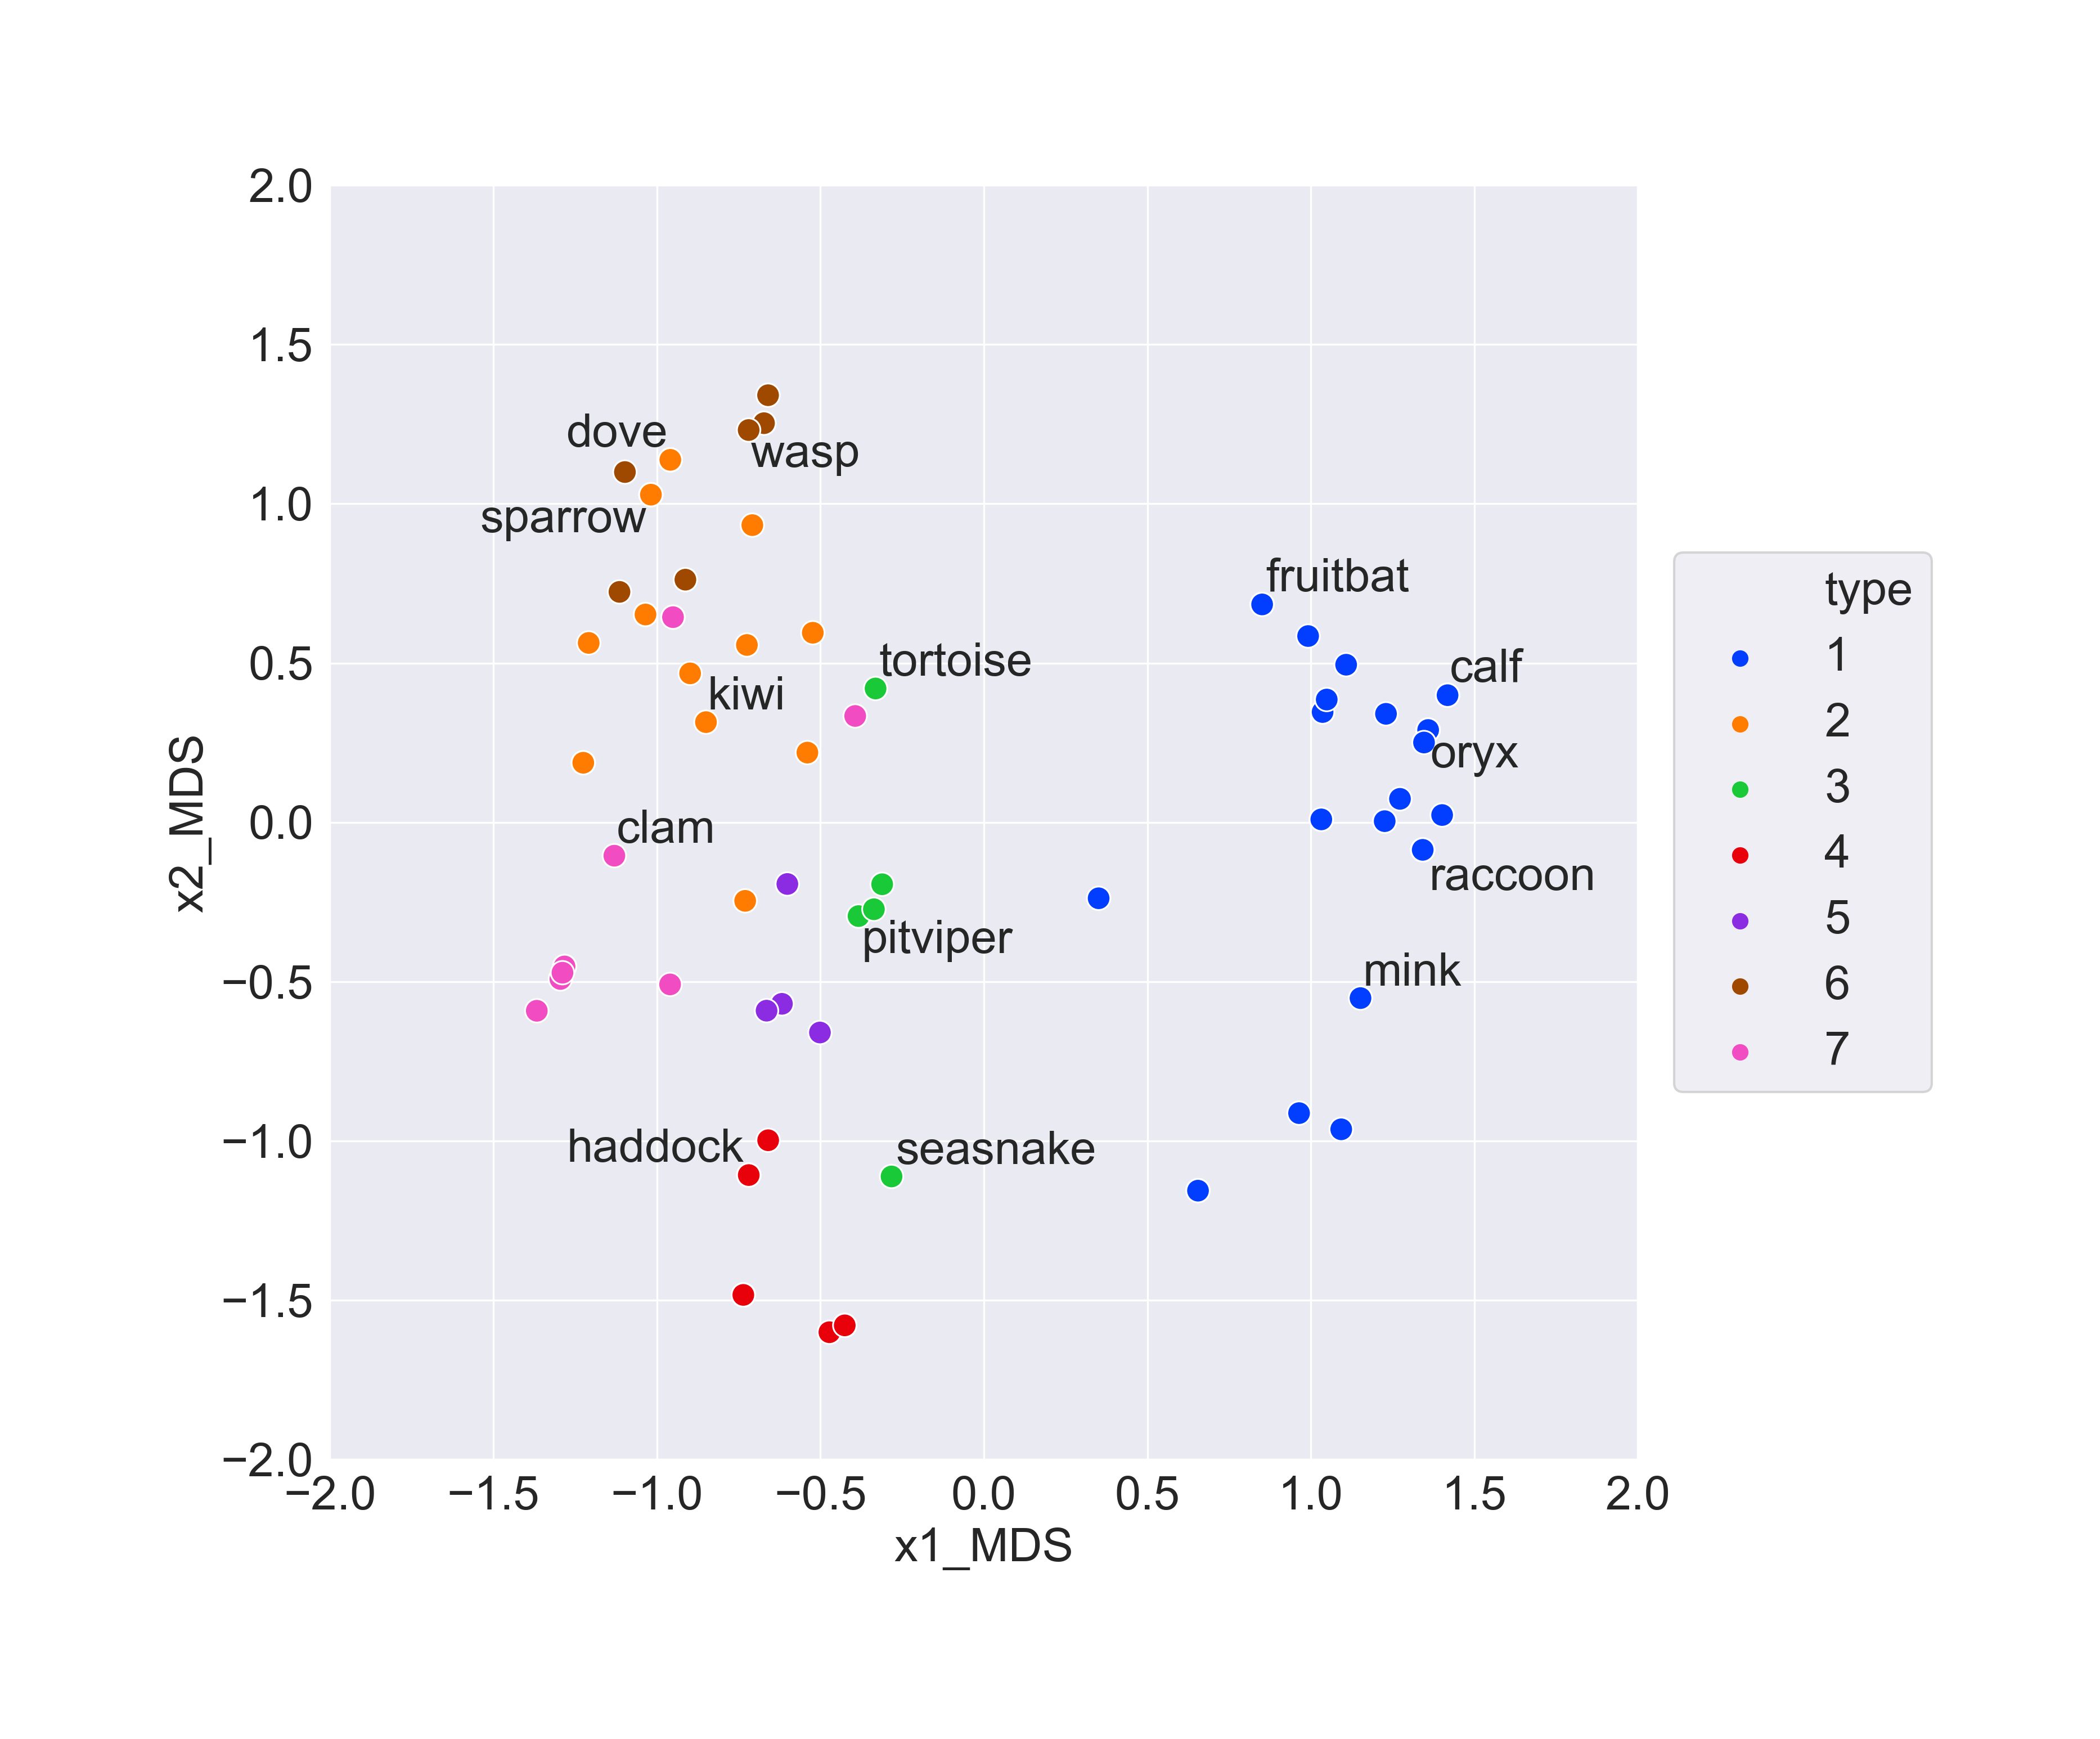
\includegraphics[width=\textwidth]{../Visualization_MDS_no_weights.png}
       \caption{All weights equal to $1$}
       \label{fig:vis_MDS1}
   \end{subfigure}
   \hspace{\fill}
   \begin{subfigure}[b]{0.6\linewidth}
       \centering
       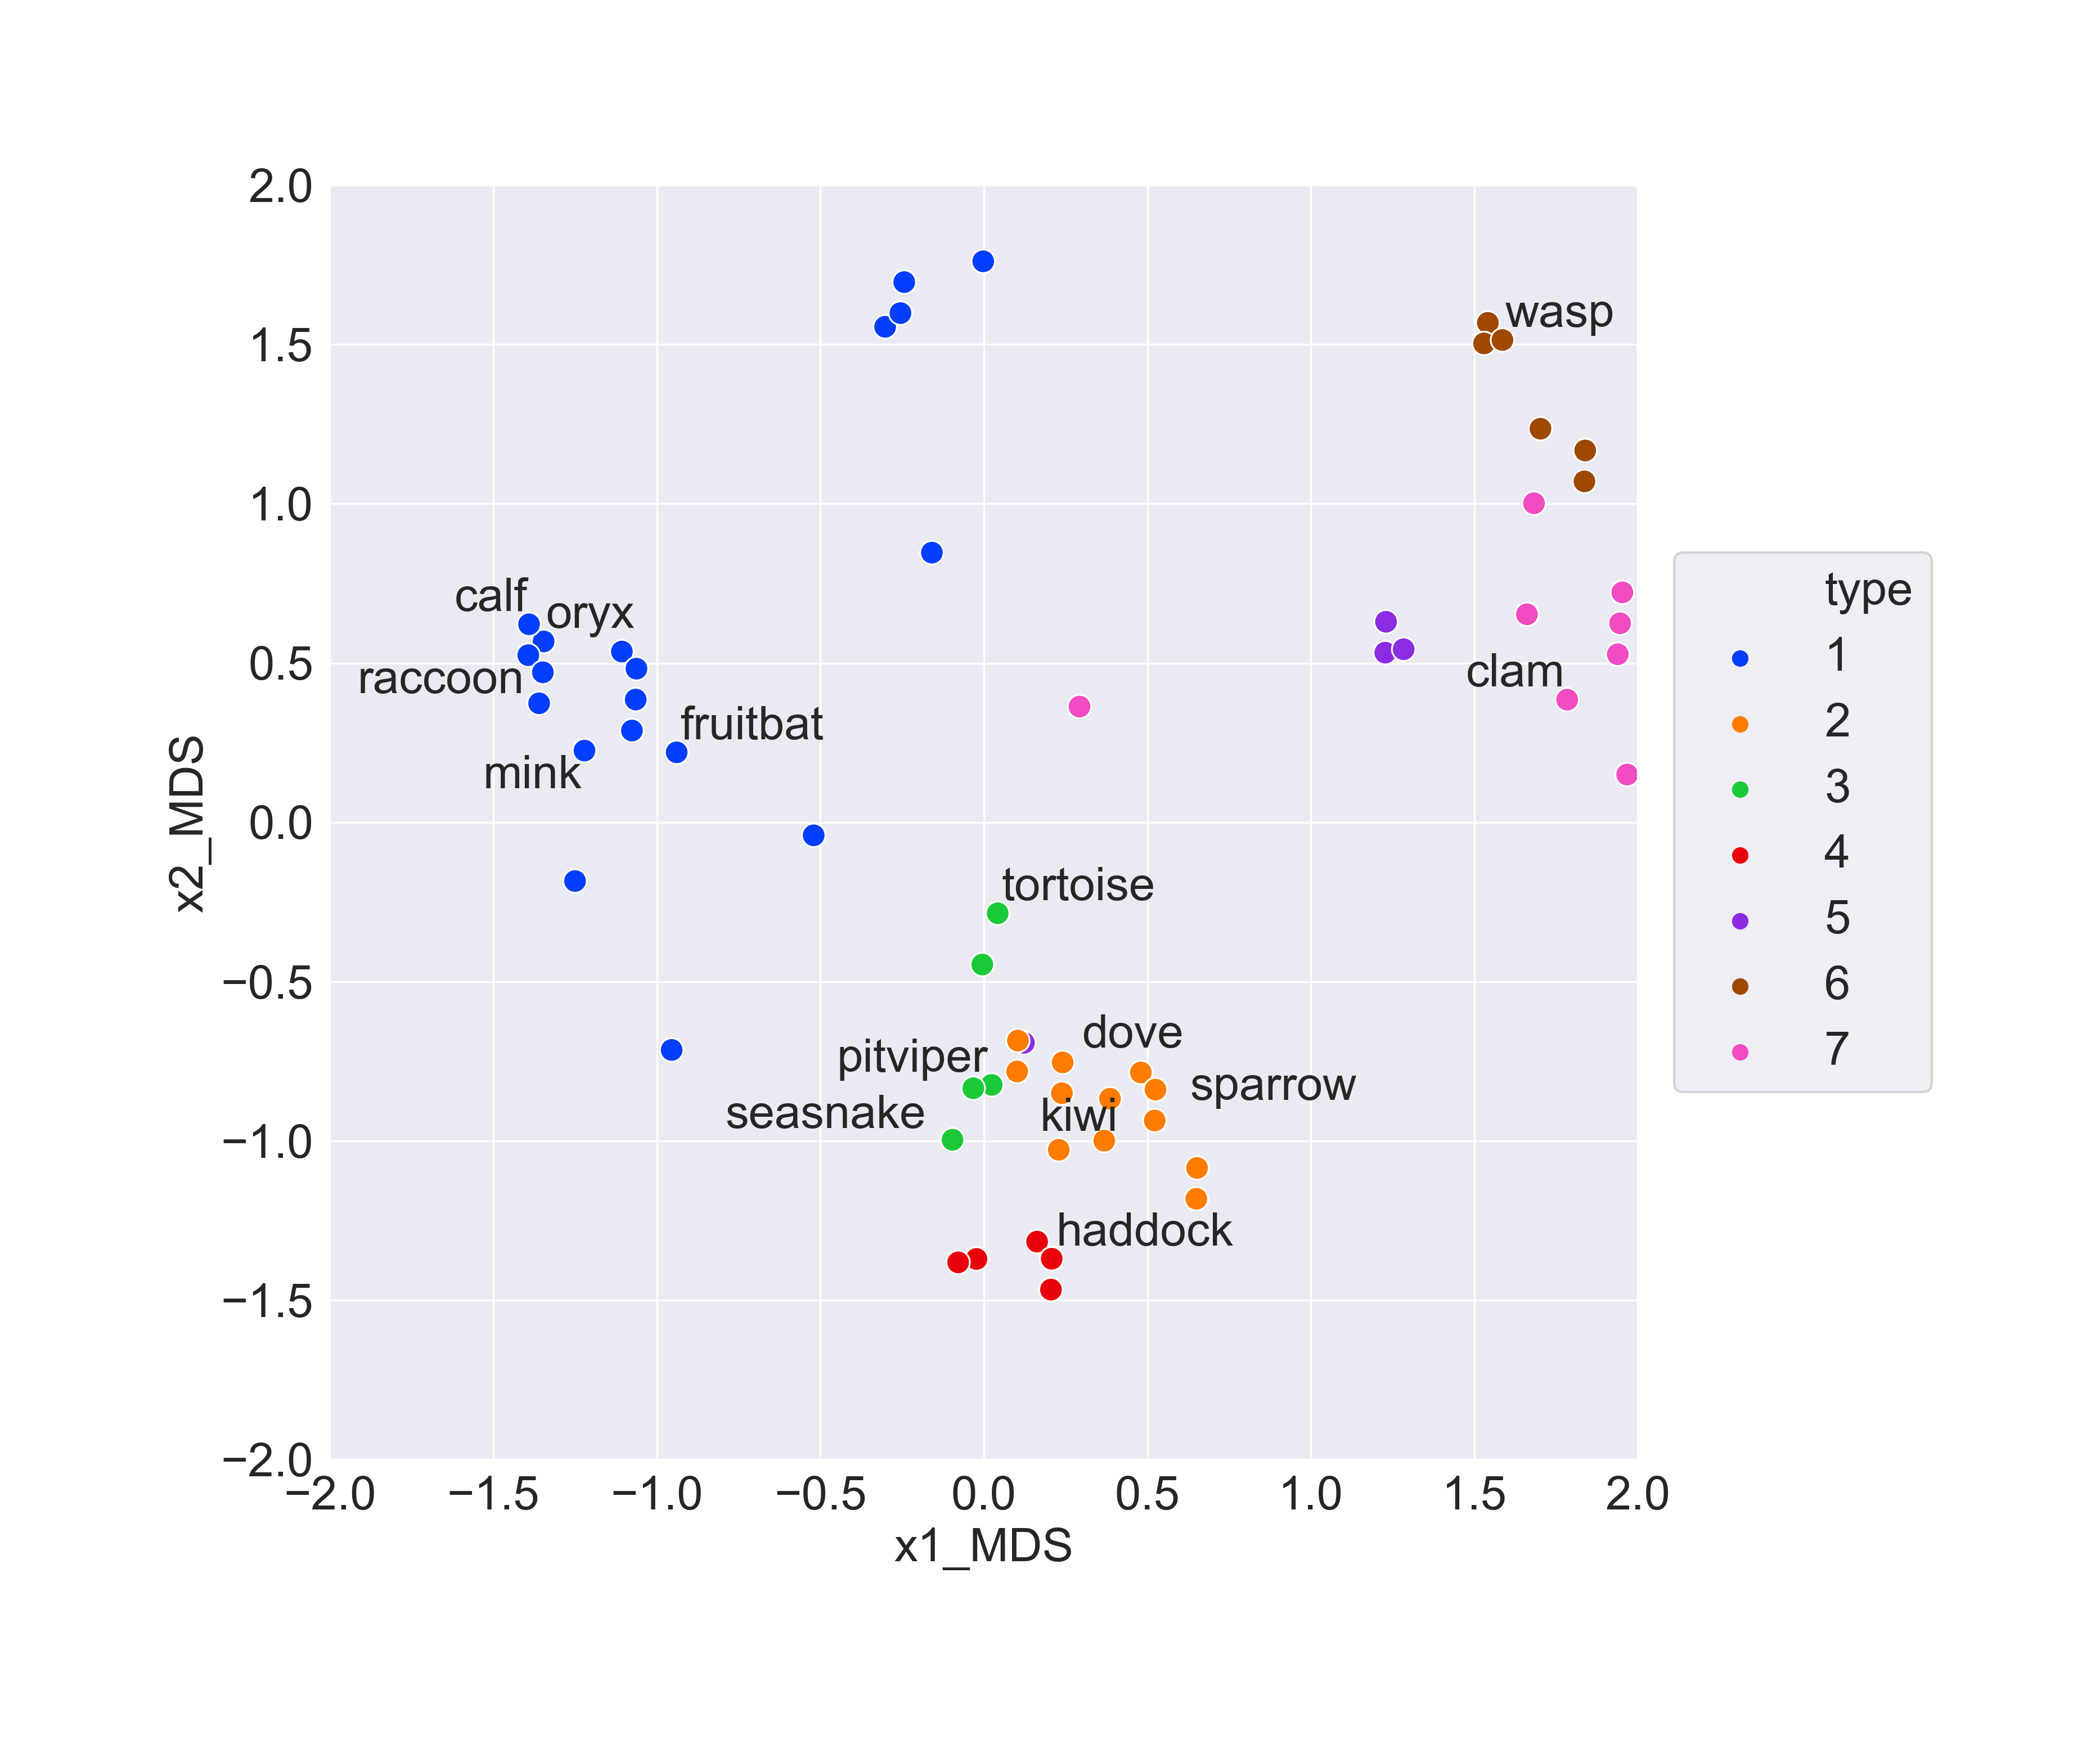
\includegraphics[width=\textwidth]{../Visualization_MDS_with_weights.png}
       \caption{$w_{legs} = 4, \; w_{tail} = 4$, rest equal to $1$}
       \label{fig:vis_MDS2}
   \end{subfigure}
      \caption{MDS method}
      \label{fig:MDS}

\end{figure}
In (\ref{fig:vis_MDS1}) one can see that using all weights equal to $1$ yields a very similar result to the one of PCA only that the points are mirrored over both the y and x axis which I believe is a result of the eigenvalue algorithm of Numpy since one can change the sign of an eigenvector and it still fulfils the eigenvalue equation.

In (\ref{fig:vis_MDS2}) the results become a bit more interesting where I have chosen to put more weight into the number of legs an animal has and whether or not it is has a tail. This has caused further separation of the data and for example the cluster of type $1$ at $(-1.2,0.5)$ seems to have the primal commonality that they all have tails (apparently a fruit bat has a tail) and secondly that they have four legs with the exception of the fruit bat which I believe is why it is in the outer proximity of the cluster.


\subsection*{Isomap}
The implementation of Isomap was solved in the following manner

\begin{algorithm}[H]
\SetAlgoLined
\KwInput{Data matrix $Y$}
\KwOutput{2-dimensional embedding $X$ }
\KwData{Zoo animals}
  Select number of neighbours $k$

  Compute a graph matrix: $G \gets \text{graph\_matrix}(\text{data matrix}, k)$

  Compute shortest path matrix: $P \gets \text{shortest\_path(G)}$

  Compute similarity matrix: $S \gets \text{similarity\_matrix} (P)$

  Compute embedding: $X \gets \text{MDS}(S)$
 \caption{Isomap method}
\end{algorithm}

In order to find the shortest path I used SciPy's implementation of the graph shortest path where I noticed even though all possible neighbours were used the returning distance matrix had a small perturbation in relation to the original distance matrix. A result that is unintuitive to me, however as the perturbations were small the end result was not affected.

The following visualisations were achieved
\begin{figure}[H]
   \centering
   \begin{subfigure}[b]{0.6\linewidth}
       \centering
       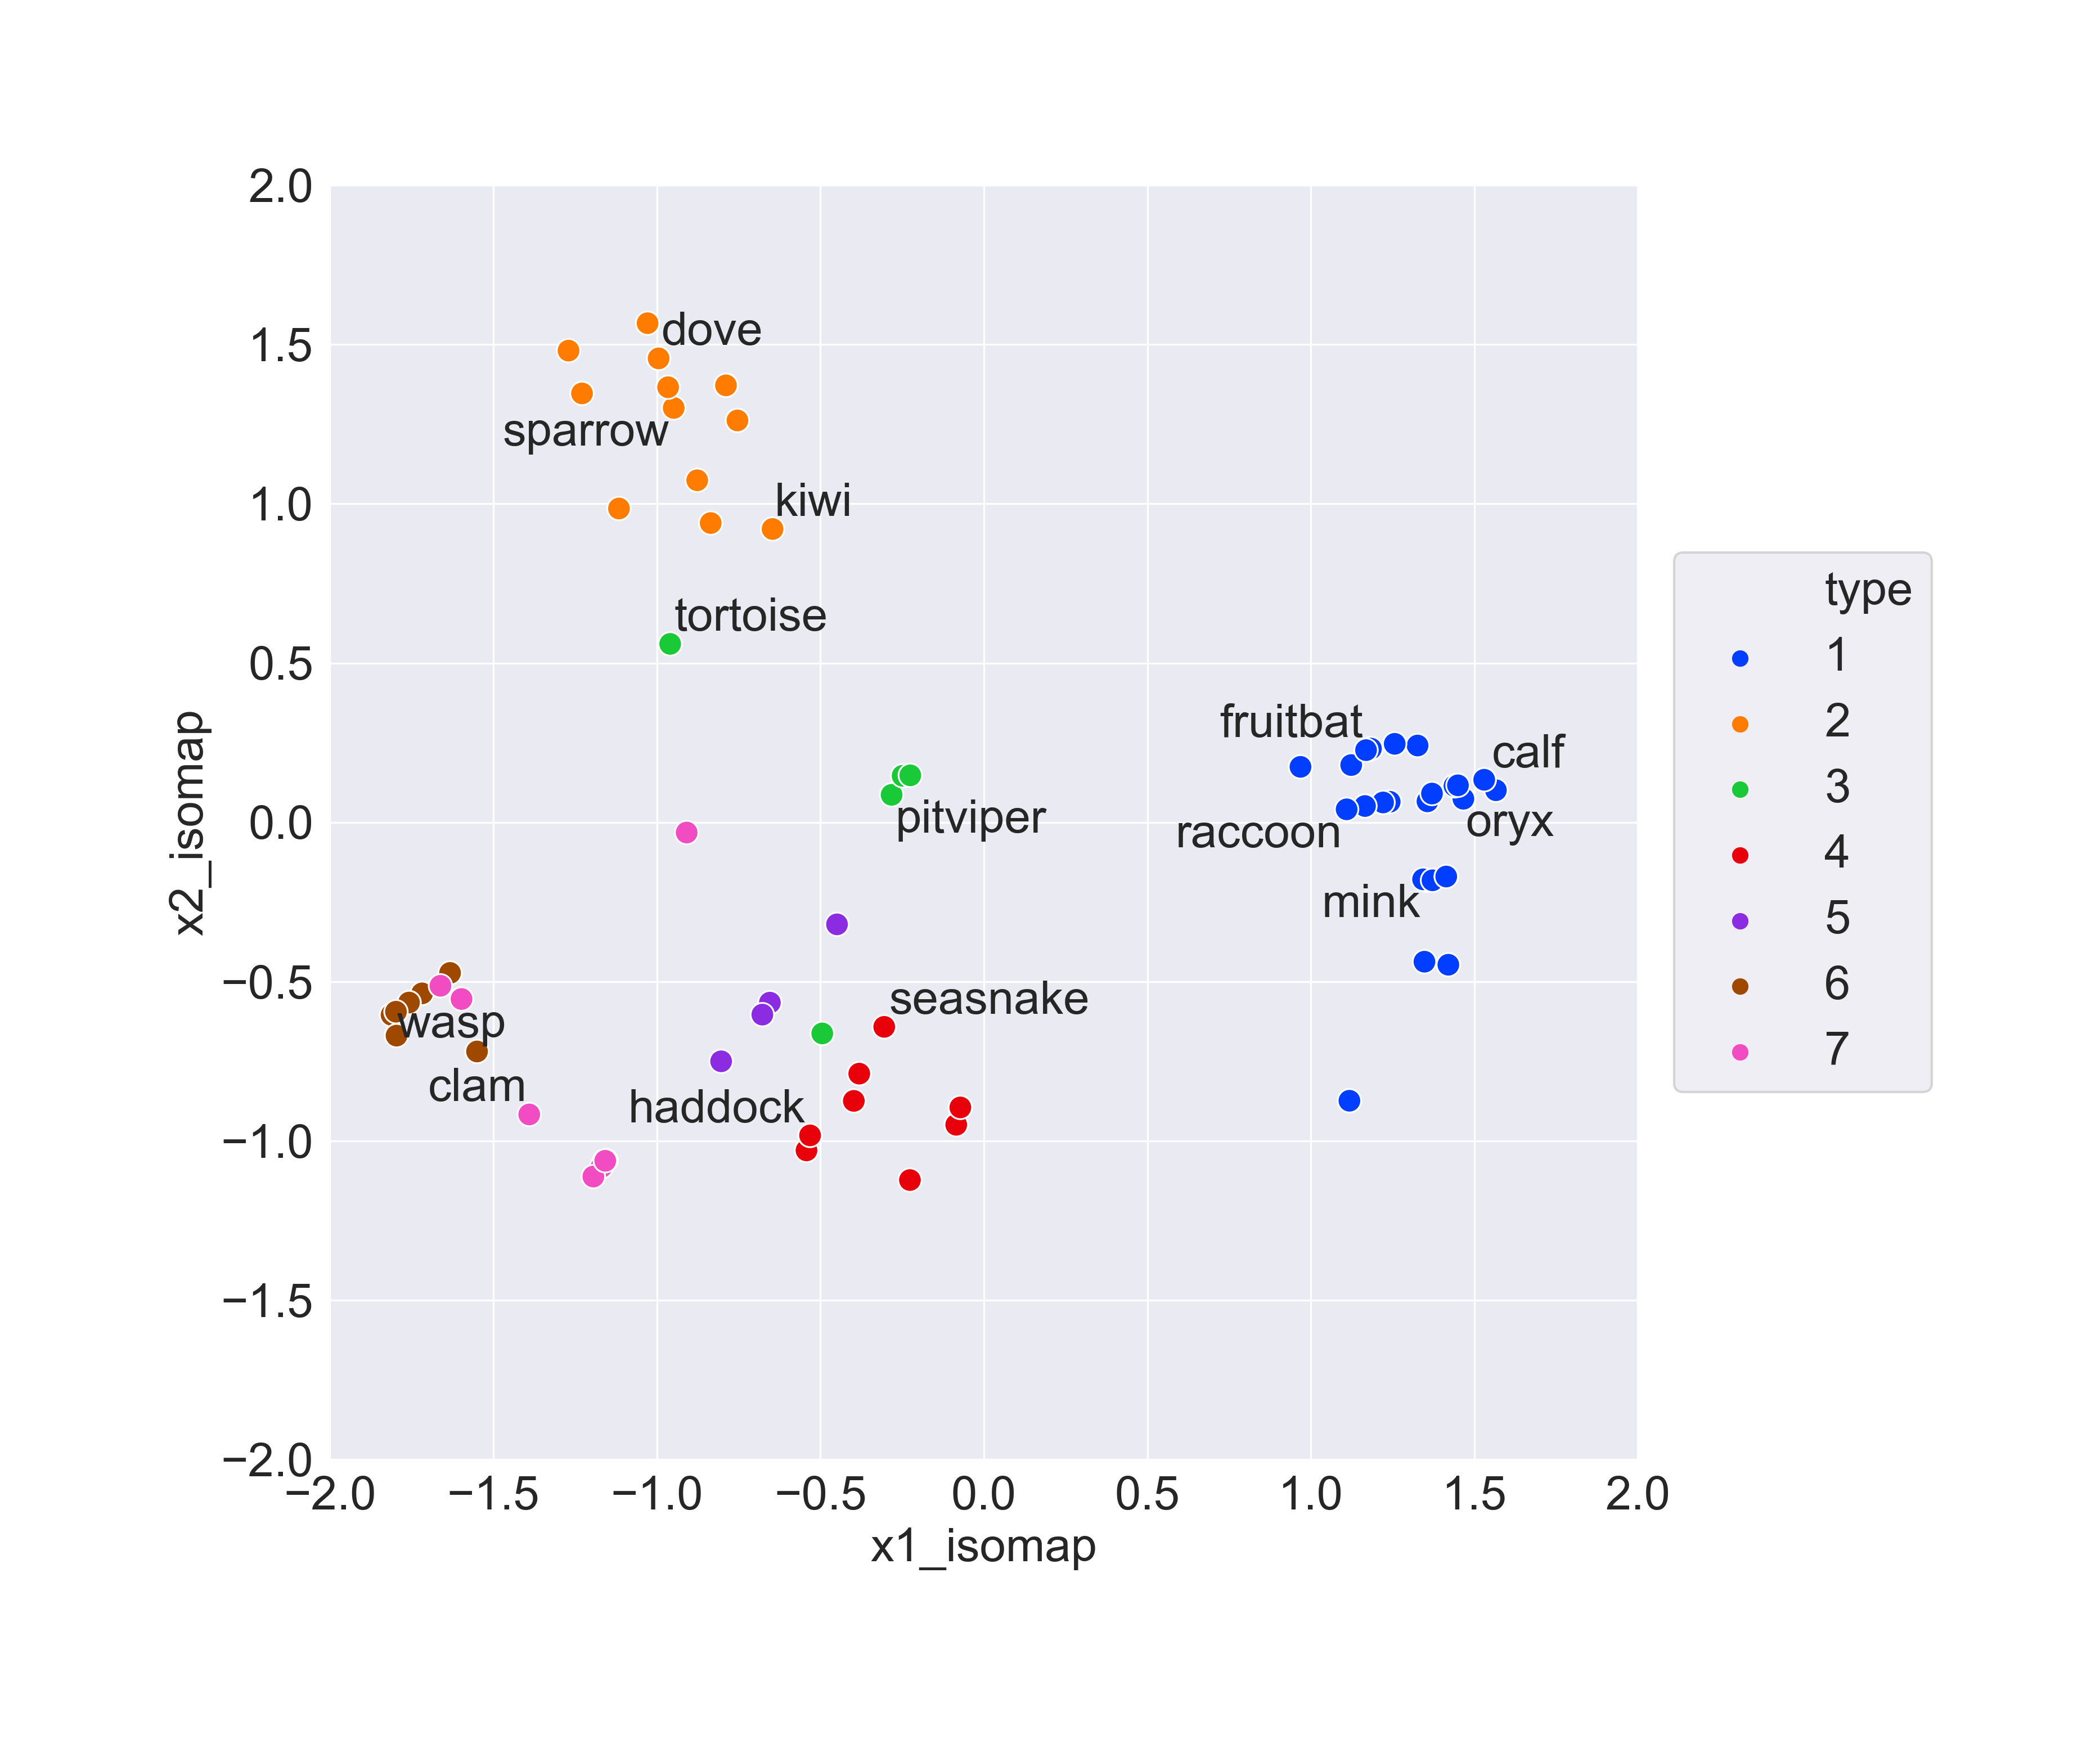
\includegraphics[width=\textwidth]{../Visualization_Isomap_n_10.png}
       \caption{Number of neighbours set to $10$}
       \label{fig:isomap 10}
   \end{subfigure}
   \hspace{\fill}
   \begin{subfigure}[b]{0.6\linewidth}
       \centering
       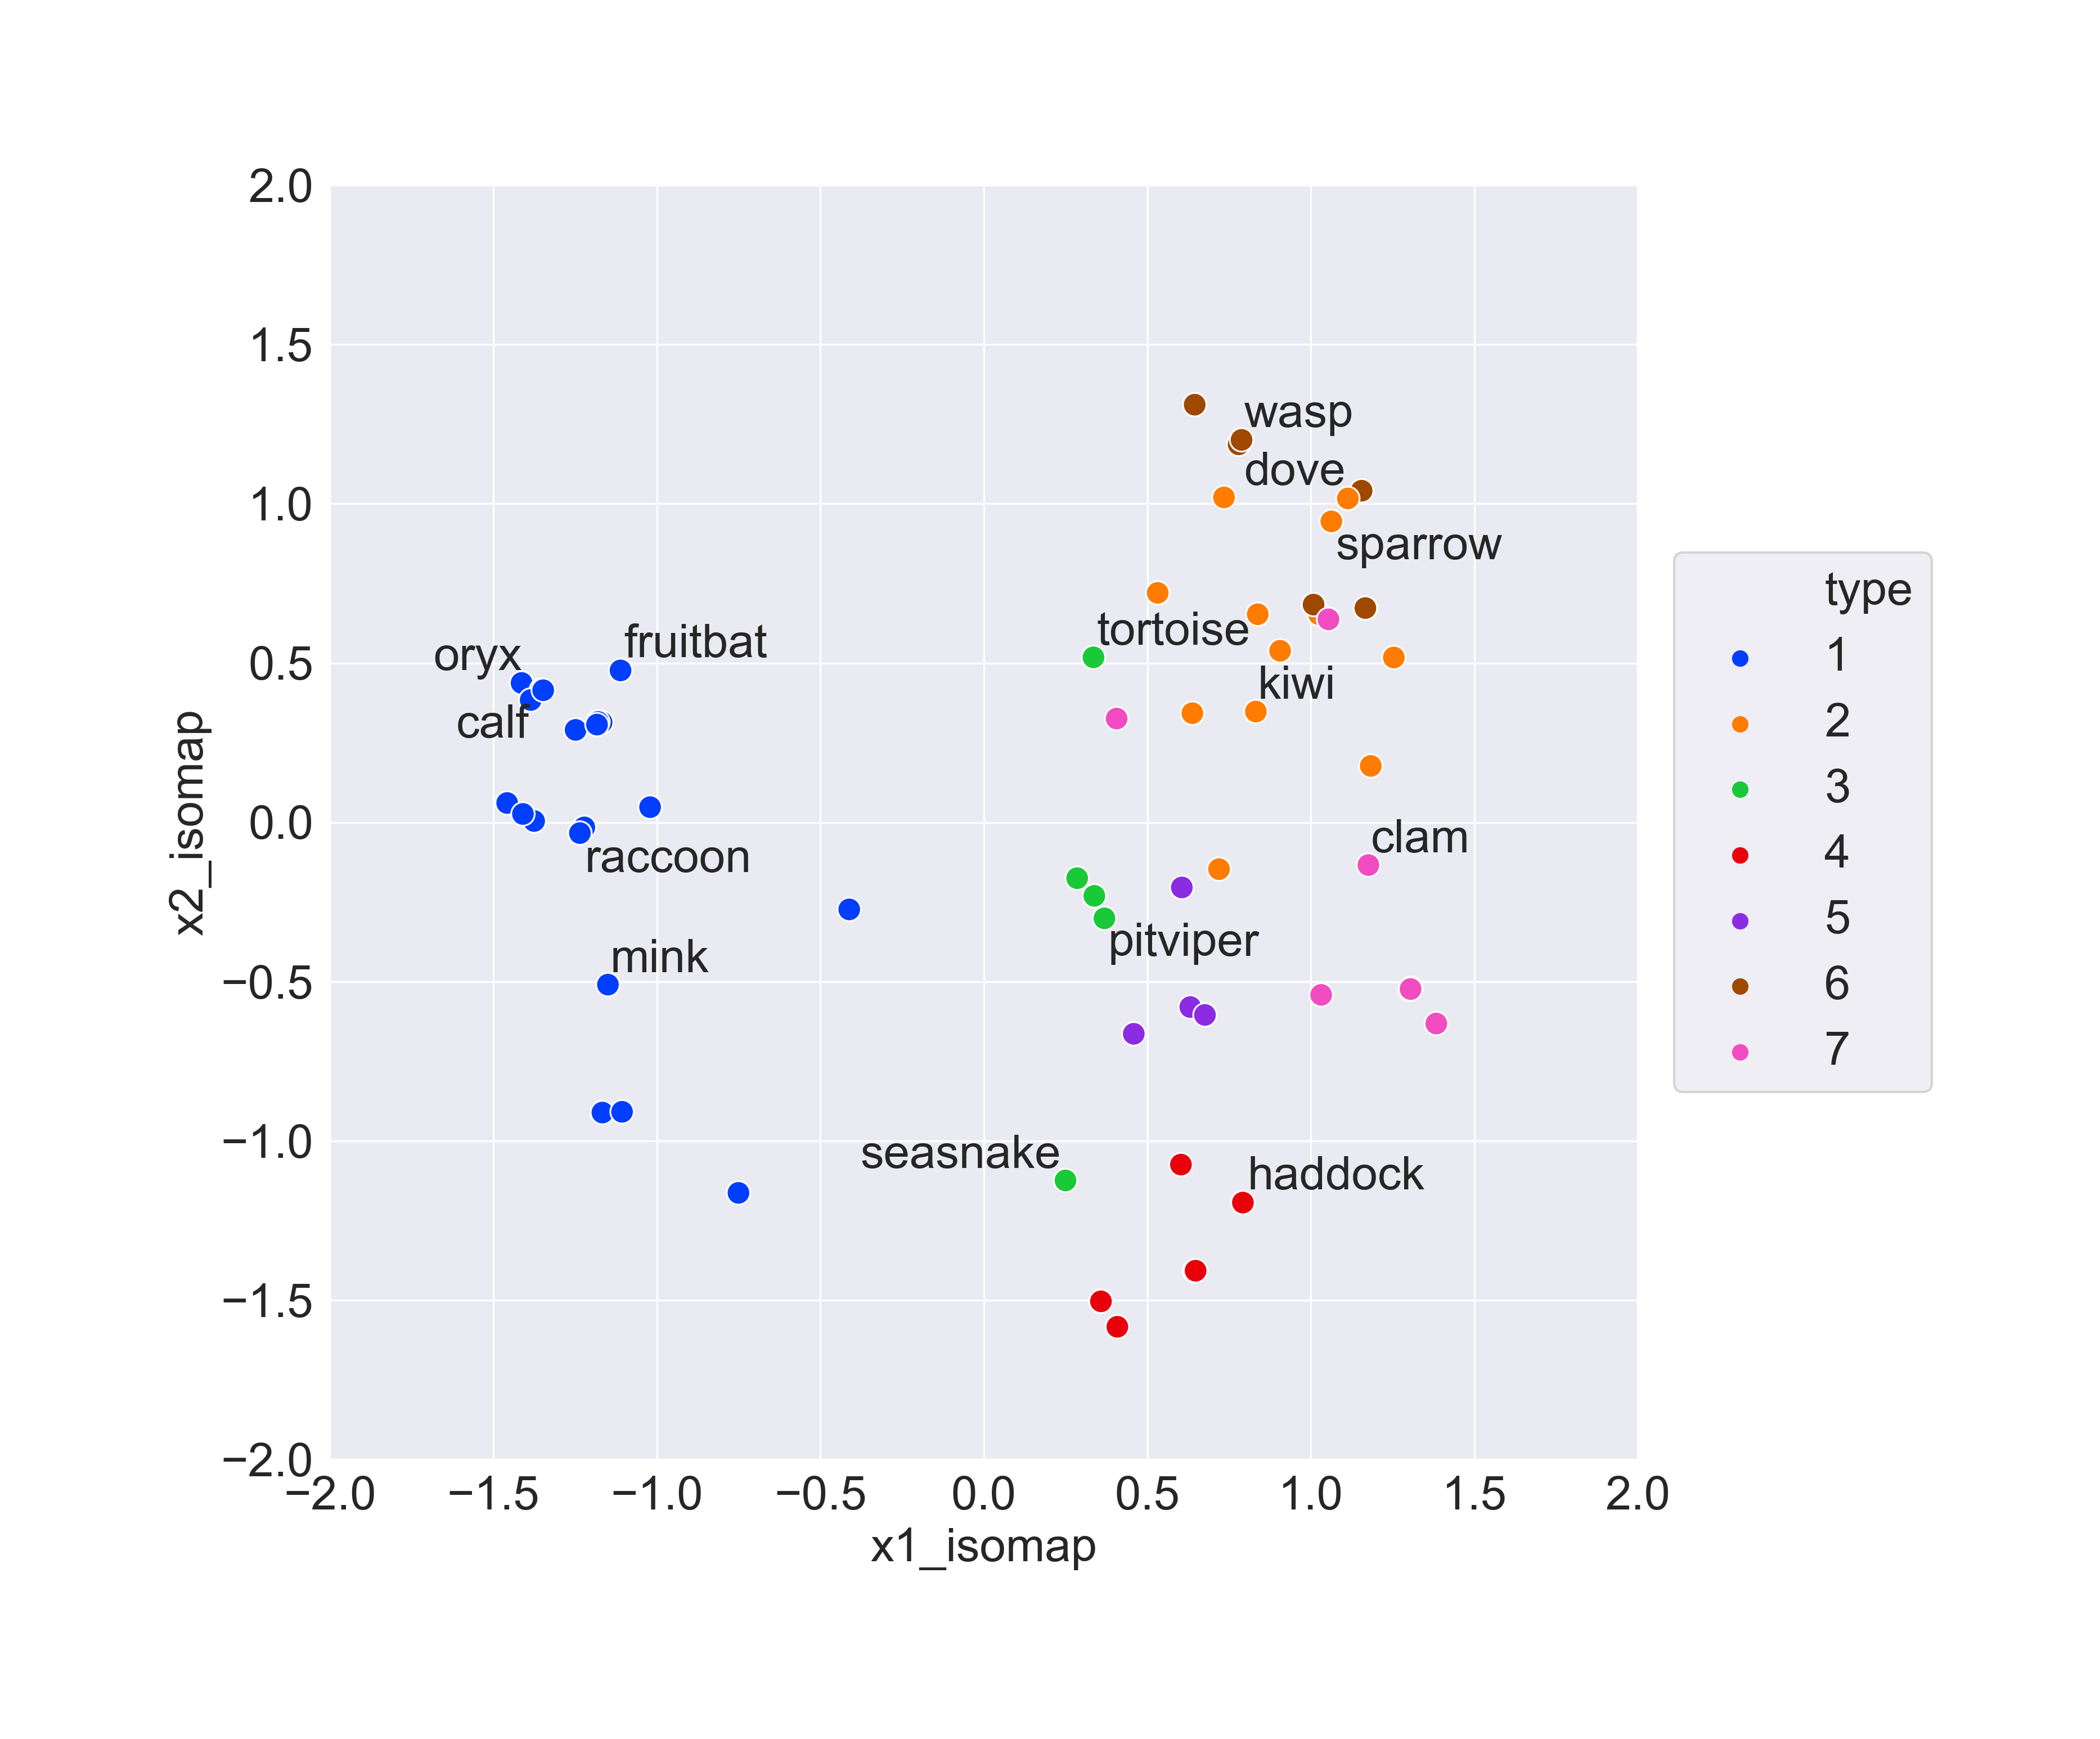
\includegraphics[width=\textwidth]{../Visualization_Isomap_n_30.png}
       \caption{Number of neighbours set to $30$}
       \label{fig:isomap 30}
   \end{subfigure}
      \caption{Isomap method}
      \label{fig:isomap}

\end{figure}

As I mentioned previously Isomap converges to the same result as both MDS and PCA (although with small perturbations) when the number of neighbours are increased. This behaviour can be seen in figure (\ref{fig:isomap 30}) where it has started to converge towards figure (\ref{fig:vis_MDS1}) where MDS has uniform weights. For this reason I opted for a low amount of neighbours in order to capture the structure of the data manifold and the final choice was set to $10$ neighbours which can be seen in figure (\ref{fig:isomap 10}). In figure (\ref{fig:isomap 10}) there is great separation between the different types of animals which gives reason to believe that Isomap captures the underlying structure of the data really well.


\subsection*{Comparison}
The final choice for each method is plotted in the three figures below.

\begin{figure}[H]
  \centering
  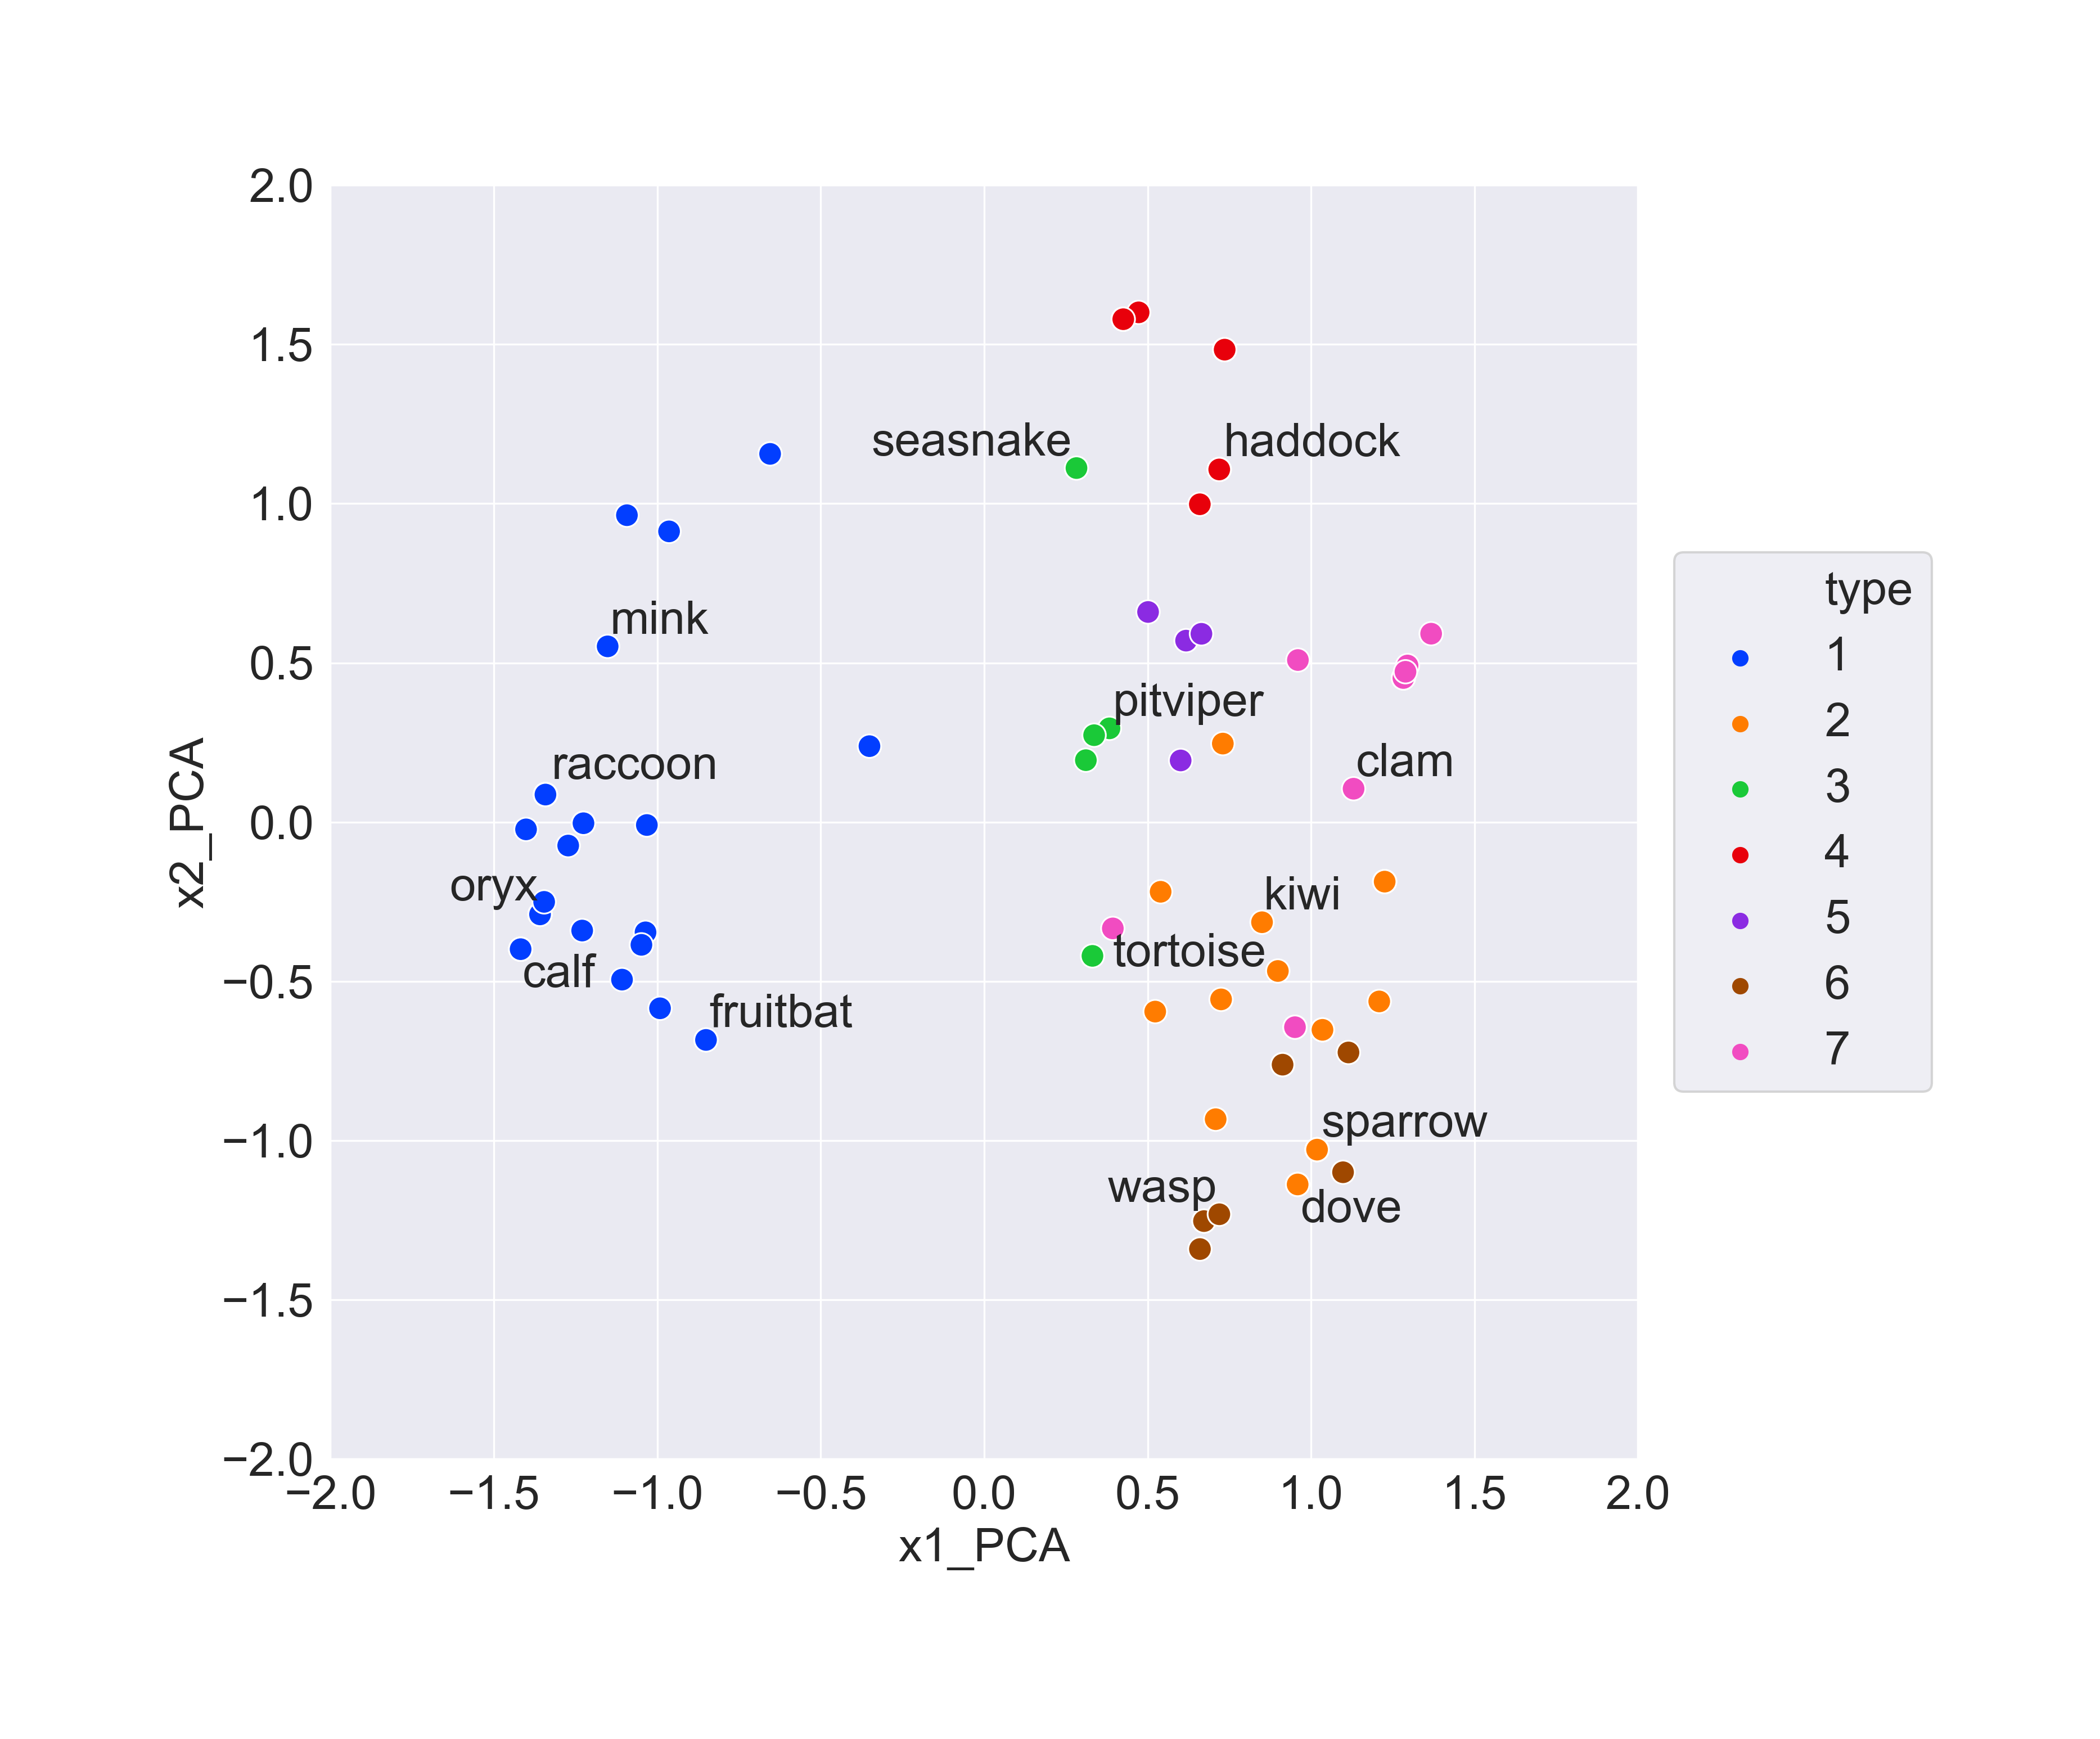
\includegraphics[width = 0.8\linewidth]{../Visualization_PCA.png}
  \caption{PCA}
  \label{fig:PCA final}
\end{figure}

\begin{figure}[H]
  \centering
  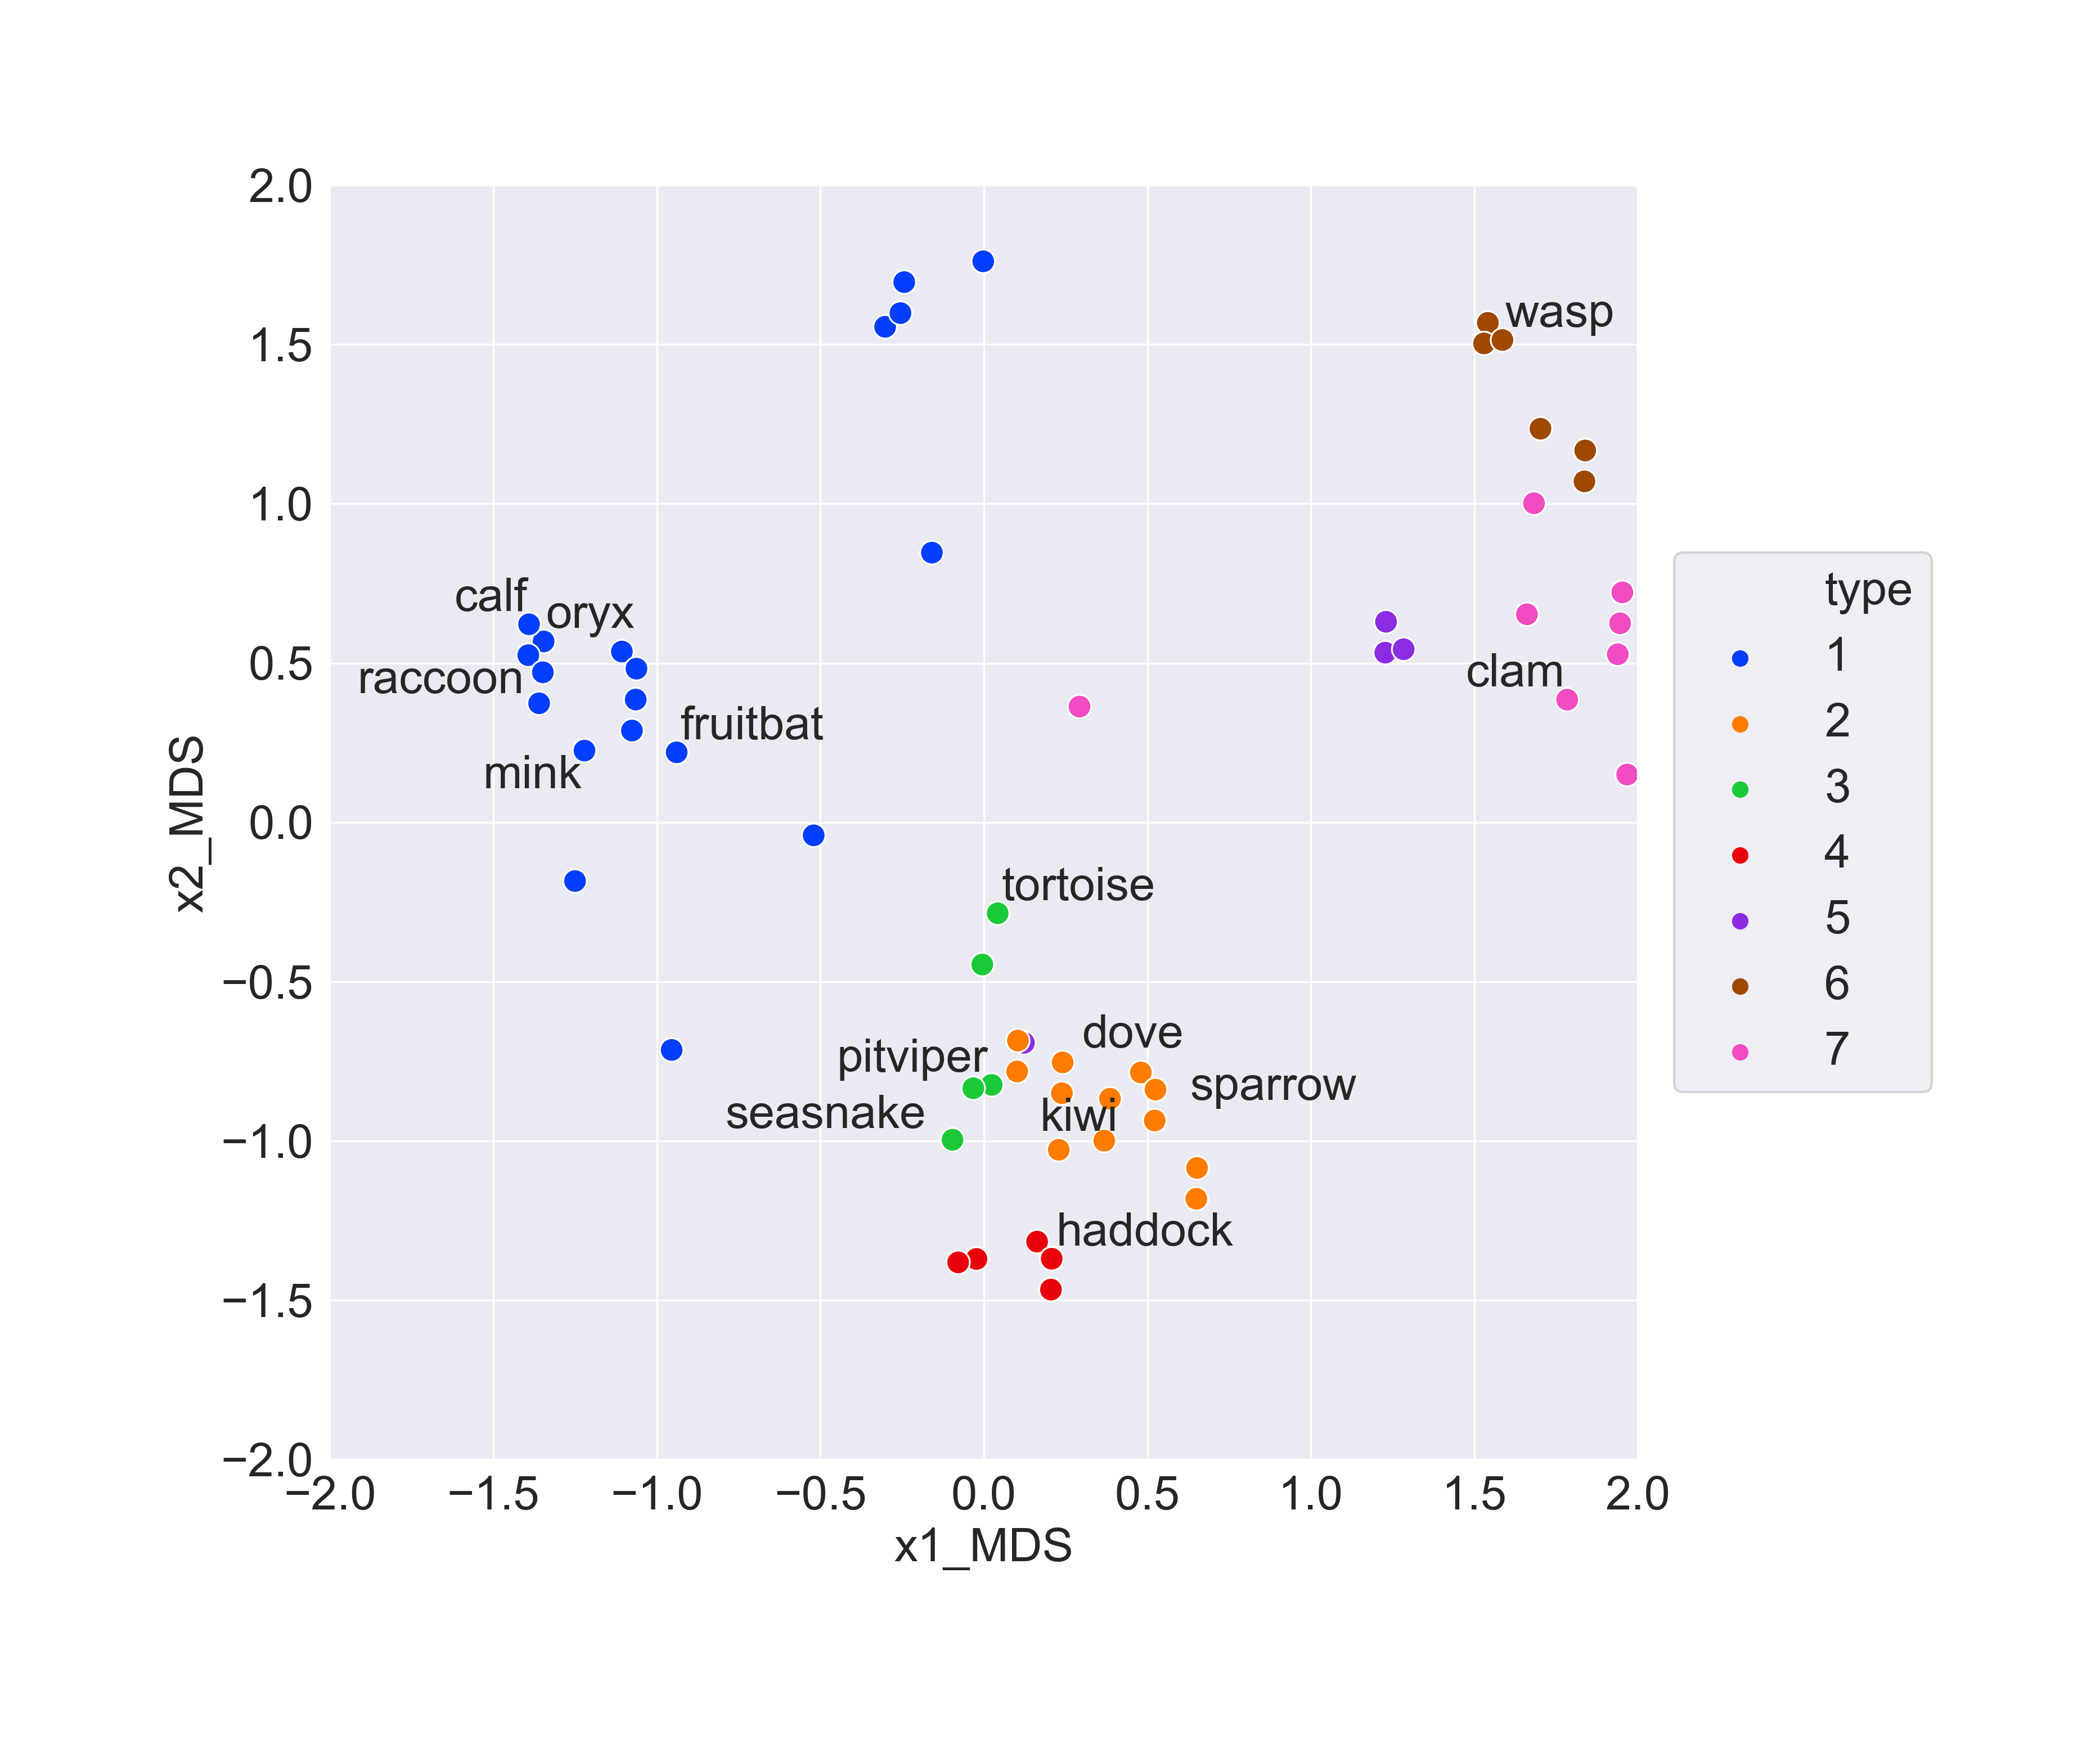
\includegraphics[width = 0.8\linewidth]{../Visualization_MDS_with_weights.png}
  \caption{MDS, $w_{legs} = 4, \; w_{tail} = 4$, rest equal to $1$}
  \label{fig:MDS final}
\end{figure}

\begin{figure}[H]
  \centering
  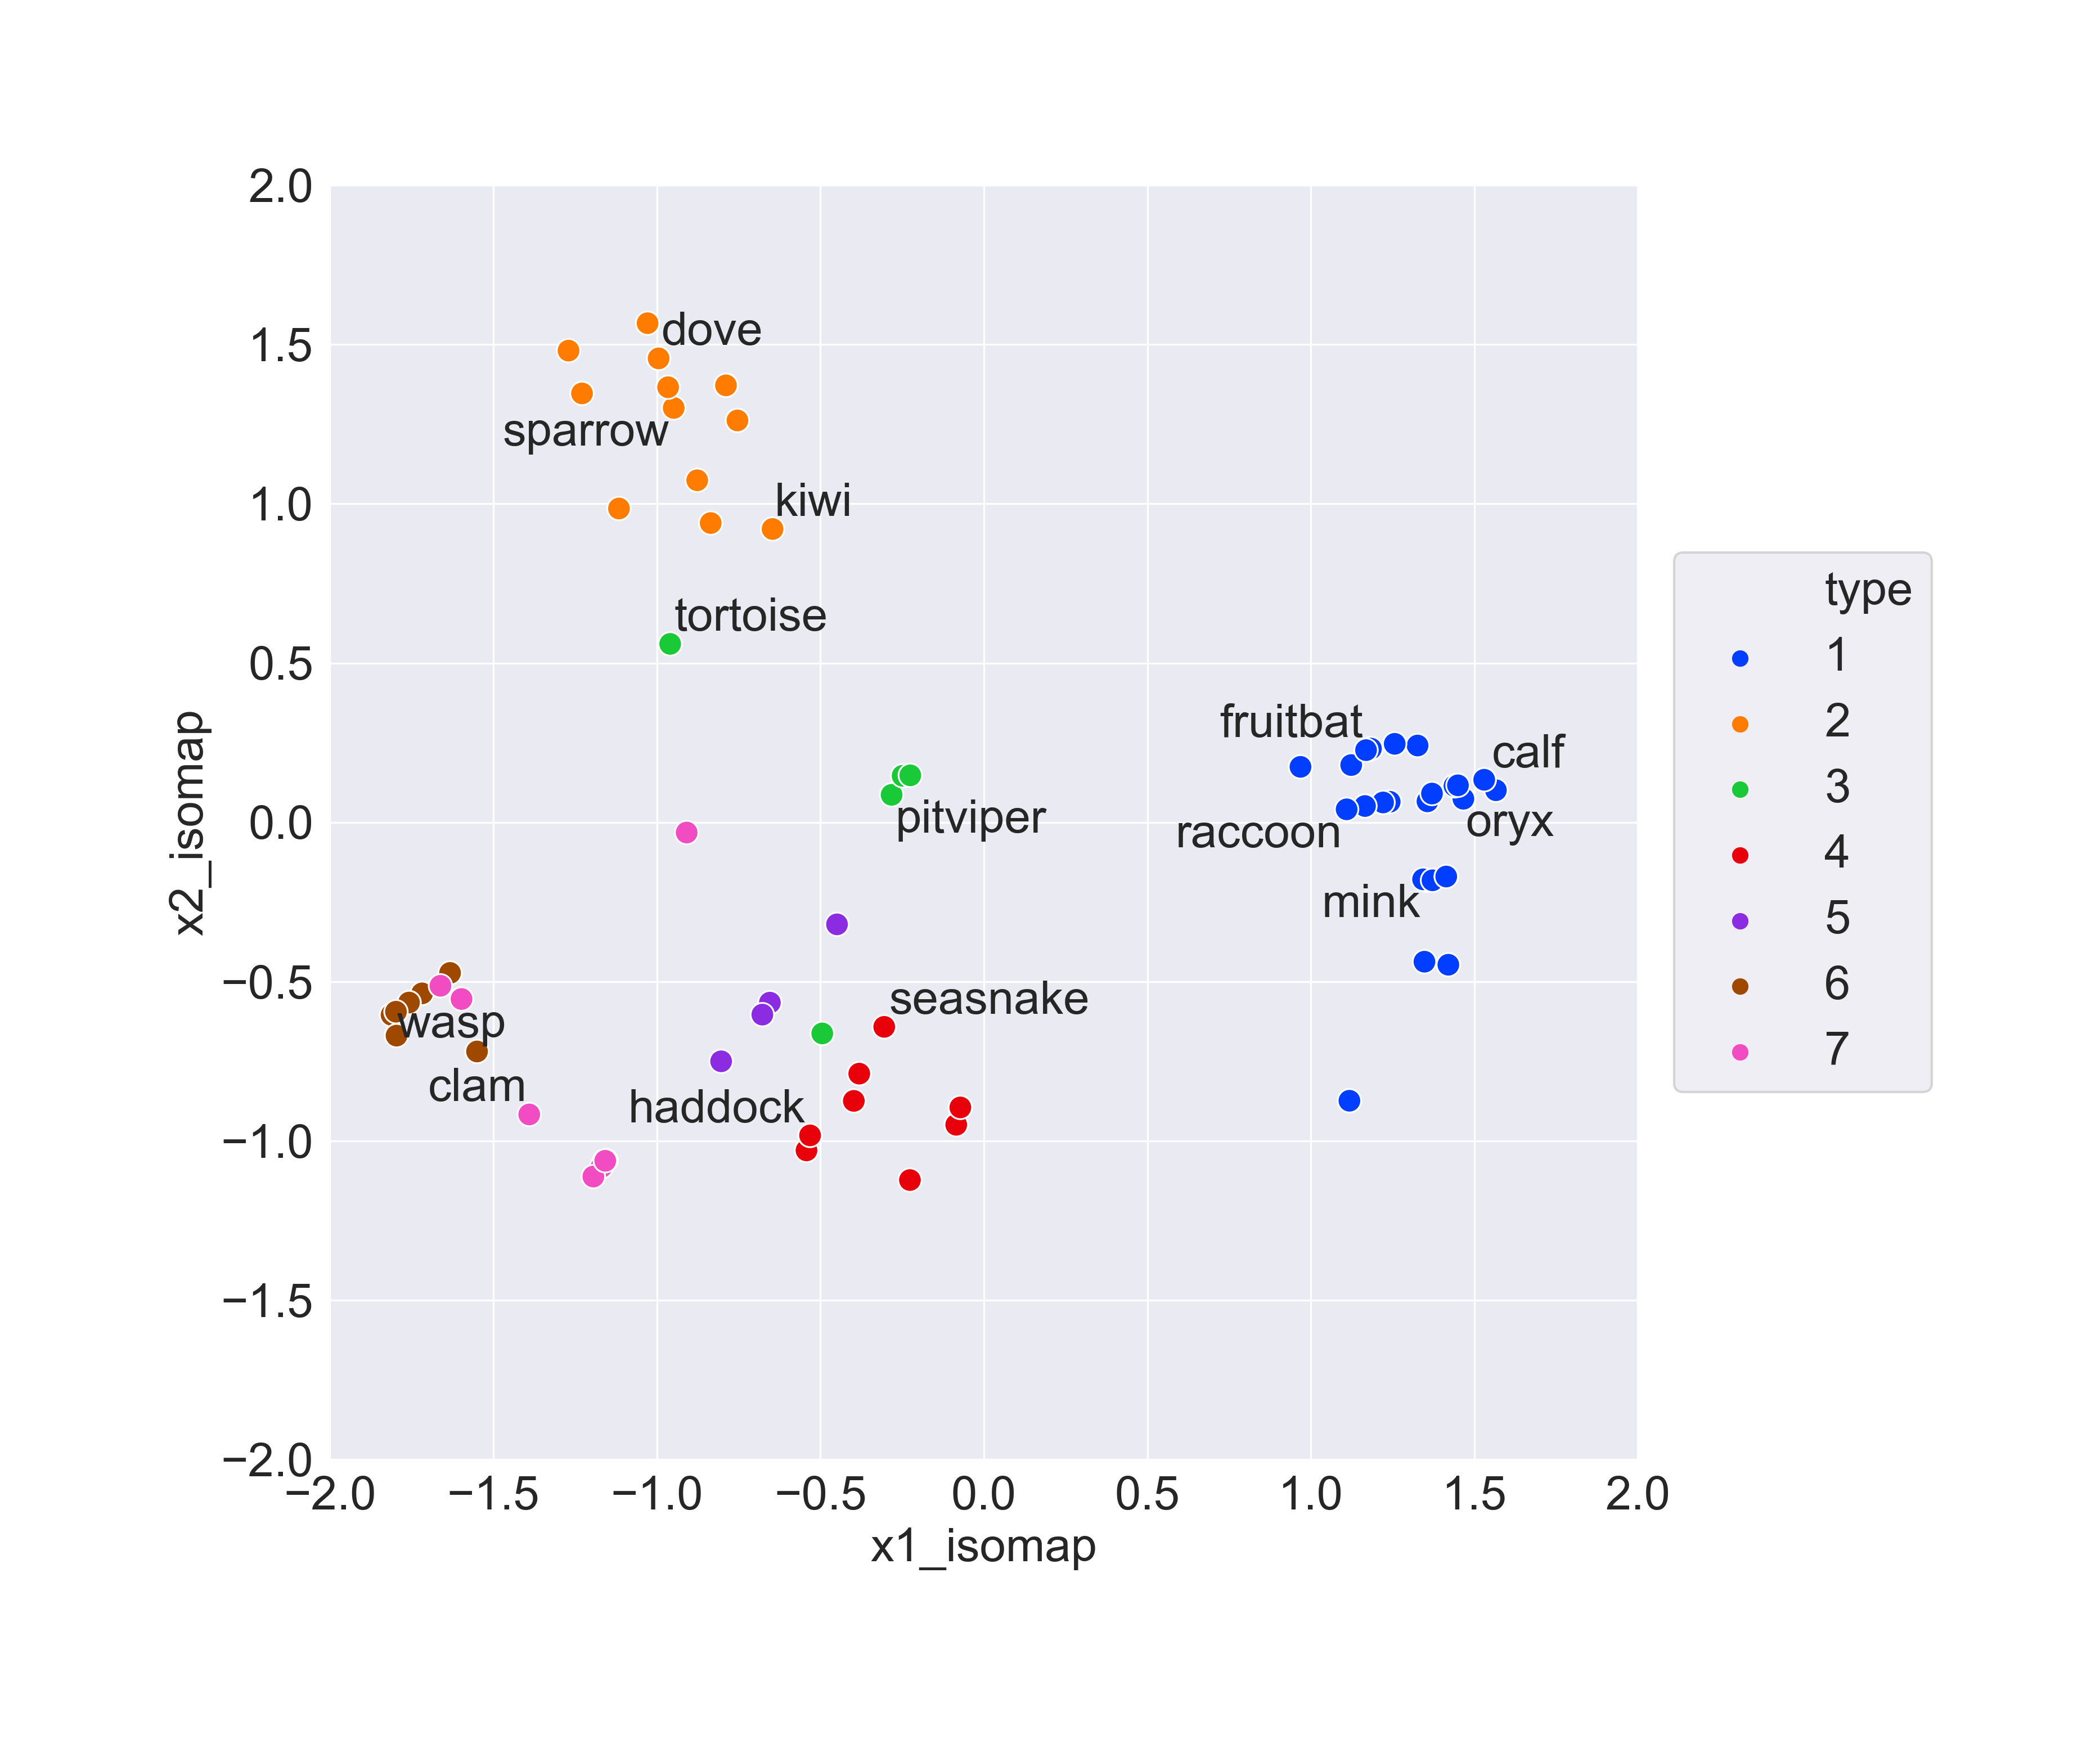
\includegraphics[width = 0.8\linewidth]{../Visualization_Isomap_n_10.png}
  \caption{Isomap, number of neighbours set to $10$}
  \label{fig:isomap 10 final}
\end{figure}

In order to make the final choice of a method I will look at how well the method captures the know relations, I.E. the relations within the designated types. This is based on the assumption that if a method correctly captures the known similarities and clusters them together it gives reason to believe that it should extrapolate well and also capture the similarities between other types of animals. Based on the plots in figures (\ref{fig:PCA final}, \ref{fig:MDS final}, \ref{fig:isomap 10 final}) Isomap perform best in clustering within types and should thus by the above assumption also be best at capturing the similarities between different types of animals. Therefore is Isomap the preferable method.


\end{document}
